\documentclass[a4paper, openright, thesis]{report}
\usepackage[fontsize=13pt]{scrextend} %dimensione font
\usepackage{comment}
\usepackage{titlesec}
\usepackage[palatino]{quotchap}
\usepackage{fancyhdr}
\usepackage{url}

\usepackage{mathptmx}
\usepackage[utf8]{inputenc} 
\usepackage[english,italian]{babel}
\usepackage{graphicx} 
\usepackage{lipsum} 
\usepackage[a4paper,top=3cm,bottom=3cm,left=3cm,right=2cm]{geometry} 
\raggedbottom 
\renewcommand{\baselinestretch}{1.5} 
\usepackage{float}
\usepackage{etoolbox}
\patchcmd{\chapter}{plain}{fancy}{}{}
\usepackage{subfigure}
\usepackage{afterpage}
\usepackage{listings}
\usepackage{xcolor}
\usepackage{hyperref}
\renewcommand{\lstlistingname}{Codice}

\definecolor{backcolor}{rgb}{0.95,0.95,0.92}
\lstdefinelanguage{JavaScript}{
    keywords={async, function, let, const, return, null, await, if, else, catch, try, throw},
    keywordstyle=\color{blue}\bfseries,
    ndkeywords={true, false, new, this},
    ndkeywordstyle=\color{teal}\bfseries,
    identifierstyle=\color{black},
    sensitive=true,
    comment=[l]{//},
    morecomment=[s]{/*}{*/},
    commentstyle=\color{gray}\itshape,
    stringstyle=\color{red},
    morestring=[b]',
    morestring=[b]"
}

\lstdefinestyle{customJS}{
    language=JavaScript,
    backgroundcolor=\color{backcolor},
    basicstyle=\ttfamily\footnotesize,
    keywordstyle=\color{blue}\bfseries,
    stringstyle=\color{red},
    commentstyle=\color{gray}\itshape,
    showstringspaces=false,
    numbers=left,
    numberstyle=\tiny\color{gray},
    frame=none,
    breaklines=true,
    tabsize=2,
    captionpos=b
}


\newcommand\blankpage{%
    \null
    \thispagestyle{empty}%
    \addtocounter{page}{-1}%
    \newpage}

\pagestyle{fancy}
\rhead{\thepage}
\cfoot{}

\begin{document}
\afterpage{\blankpage}
\newpage
\renewcommand{\baselinestretch}{1} 

\begin{titlepage}
\begin{figure}[!htb]
    \centering
    
\includegraphics[width=7cm]{unifi.png}
\end{figure}

\begin{center}
    \LARGE{UNIVERSITÀ DI FIRENZE}
    \vspace{4mm}
    \\ \large{DIPARTIMENTO DI INGEGNERIA DELL'INFORMAZIONE }
    \vspace{4mm}
    \\ \LARGE{Corso di Laurea Triennale in Ingegneria Informatica}
\end{center}

\vspace{15mm}
\begin{center}
    {\LARGE{\bf Soluzioni Scalabili per l'Analisi degli Eventi Urbani tramite l'Integrazione di Snap4City e Sistemi di Gestione Video}}
\end{center}
\vspace{25mm}

\begin{minipage}[t]{0.5\textwidth}
	{\large{Relatori:}{\normalsize
	\bf\\ \large{Nesi Paolo\\Luciano Alessandro Ipsaro Palesi}}}
\end{minipage}
\hfill
\begin{minipage}[t]{0.45\textwidth}\raggedleft
	{\large{Candidato:}{\normalsize\vspace{3mm} \bf\\ \large{Angeli Giovanni\\ }}}
\end{minipage}

\vspace{10mm}
\hrulefill
\\\centering{\large{ANNO ACCADEMICO 2023/2024}}

\end{titlepage}


\pagenumbering{Roman} 


\chapter*{Ringraziamenti}

\tableofcontents

\afterpage{\blankpage}
\newpage

\pagenumbering{arabic} 
\setcounter{page}{1}


\chapter{INTRODUZIONE}

L’obiettivo della tesi consiste nello studio e lo sviluppo di una soluzione scalabile orientata all'analisi di eventi urbani tramite l'integrazione di un complesso di telecamere termiche con la
piattaforma Snap4city \cite{snap4city} in modo da permettere una comunicazione biunivoca tra le due strutture.
Le telecamere sono gestite da un Video Management System (di seguito VMS), chiamato Milestone
Xprotect \cite{milestoneVMS}, che offre un’ interfaccia grafica per lo streaming video di tutte le telecamere collegate
con possibilità di registrare o di acquisire delle schermate. Inoltre, ci consente di gestire una serie di eventi e allarmi legati al funzionamento delle
telecamere oppure alle situazioni rilevate dallo streaming video, con la possibilità di far definire all’utente stesso un particolare evento o allarme. Lo scopo principale è quindi mantenere allineate entrambe le piattaforme, gestendo in maniera efficace e in tempo reale gli eventi generati sia dal VMS delle telecamere che dalla piattaforma Snap4City.

\afterpage{\blankpage}

\chapter{ANALISI DEI REQUISITI}
In questo capitolo viene effettuata un’analisi dettagliata dei requisiti necessari per la realizzazione del progetto, con l’obiettivo di definire in modo chiaro e strutturato le esigenze funzionali, architetturali e di sviluppo. Questa rappresenta un passaggio fondamentale per garantire che le soluzioni proposte siano coerenti con gli obiettivi prefissati e rispondano efficacemente alle esigenze degli utenti e dei sistemi coinvolti.

\section{Requisiti Funzionali}

Di seguito sono descritti i principali requisiti funzionali identificati per l’integrazione dei due sistemi:

\begin{itemize}
    \item \textbf{Comunicazione Biunivoca tra Sistemi:} l’integrazione deve garantire uno scambio bidirezionale di informazioni tra il VMS e la piattaforma Snap4City. Questo permetterà ai due sistemi di aggiornarsi in tempo reale, sincronizzando e propagando stati ed eventi in modo continuo e senza discrepanze operative.

    \item \textbf{Gestione Eventi e Allarmi:} un elemento fondamentale del progetto è la gestione degli eventi e degli allarmi. Il VMS dovrà notificare a Snap4City eventuali problematiche tecniche, come malfunzionamenti hardware o software, e segnalare situazioni rilevanti. Sarà inoltre possibile configurare eventi personalizzati definiti dall’utente, garantendo flessibilità e un approccio adattabile alle esigenze.

    \item \textbf{Integrazione dei Flussi Video:} è prevista l’integrazione dei dati video, includendo lo streaming in tempo reale, le registrazioni e le schermate catturate. Questi dati potranno essere utilizzati per analisi dettagliate o per la generazione di report. Sarà altresì importante assicurare una gestione efficace dello storico delle registrazioni, rispettando le normative sulla conservazione dei dati e facilitando l’accesso alle informazioni archiviate.

    \item \textbf{Dashboard per gli operatori:} un’interfaccia interattiva sarà sviluppata tramite Snap4City per offrire agli operatori un accesso immediato ai dati e alle situazioni più rilevanti. Le dashboard saranno progettate per semplificare il monitoraggio delle telecamere, gestire e configurare gli allarmi, visualizzare lo storico degli eventi. Saranno integrati strumenti grafici avanzati, come mappe e grafici interattivi, per rendere più intuitiva l’interpretazione dei dati e facilitare il processo decisionale.

    \item \textbf{Scalabilità e Modularità:} il sistema dovrà essere scalabile e progettato in modo modulare, per consentire l’aggiunta di nuove funzionalità o il supporto di ulteriori dispositivi senza alterare significativamente l’architettura.

    \item \textbf{Sicurezza e Affidabilità:} la sicurezza della trasmissione dei dati tra le due piattaforme sarà una priorità, da garantire tramite l’uso di protocolli cifrati che prevengano accessi non autorizzati. Parallelamente, il sistema sarà progettato per gestire errori e guasti in modo robusto, riducendo al minimo l’impatto sulle operazioni e assicurando continuità nelle funzioni critiche.
    
\end{itemize}
\newpage

\section{Architettura}
L’architettura generale dell'integrazione, rappresentata in Figura \ref{archgen} e articolata in tre macro-componenti, integra il VMS con la piattaforma Snap4City fornendo un framework modulare per la gestione degli eventi e l’analisi dei dati.
\begin{figure}[H]
    \centering
    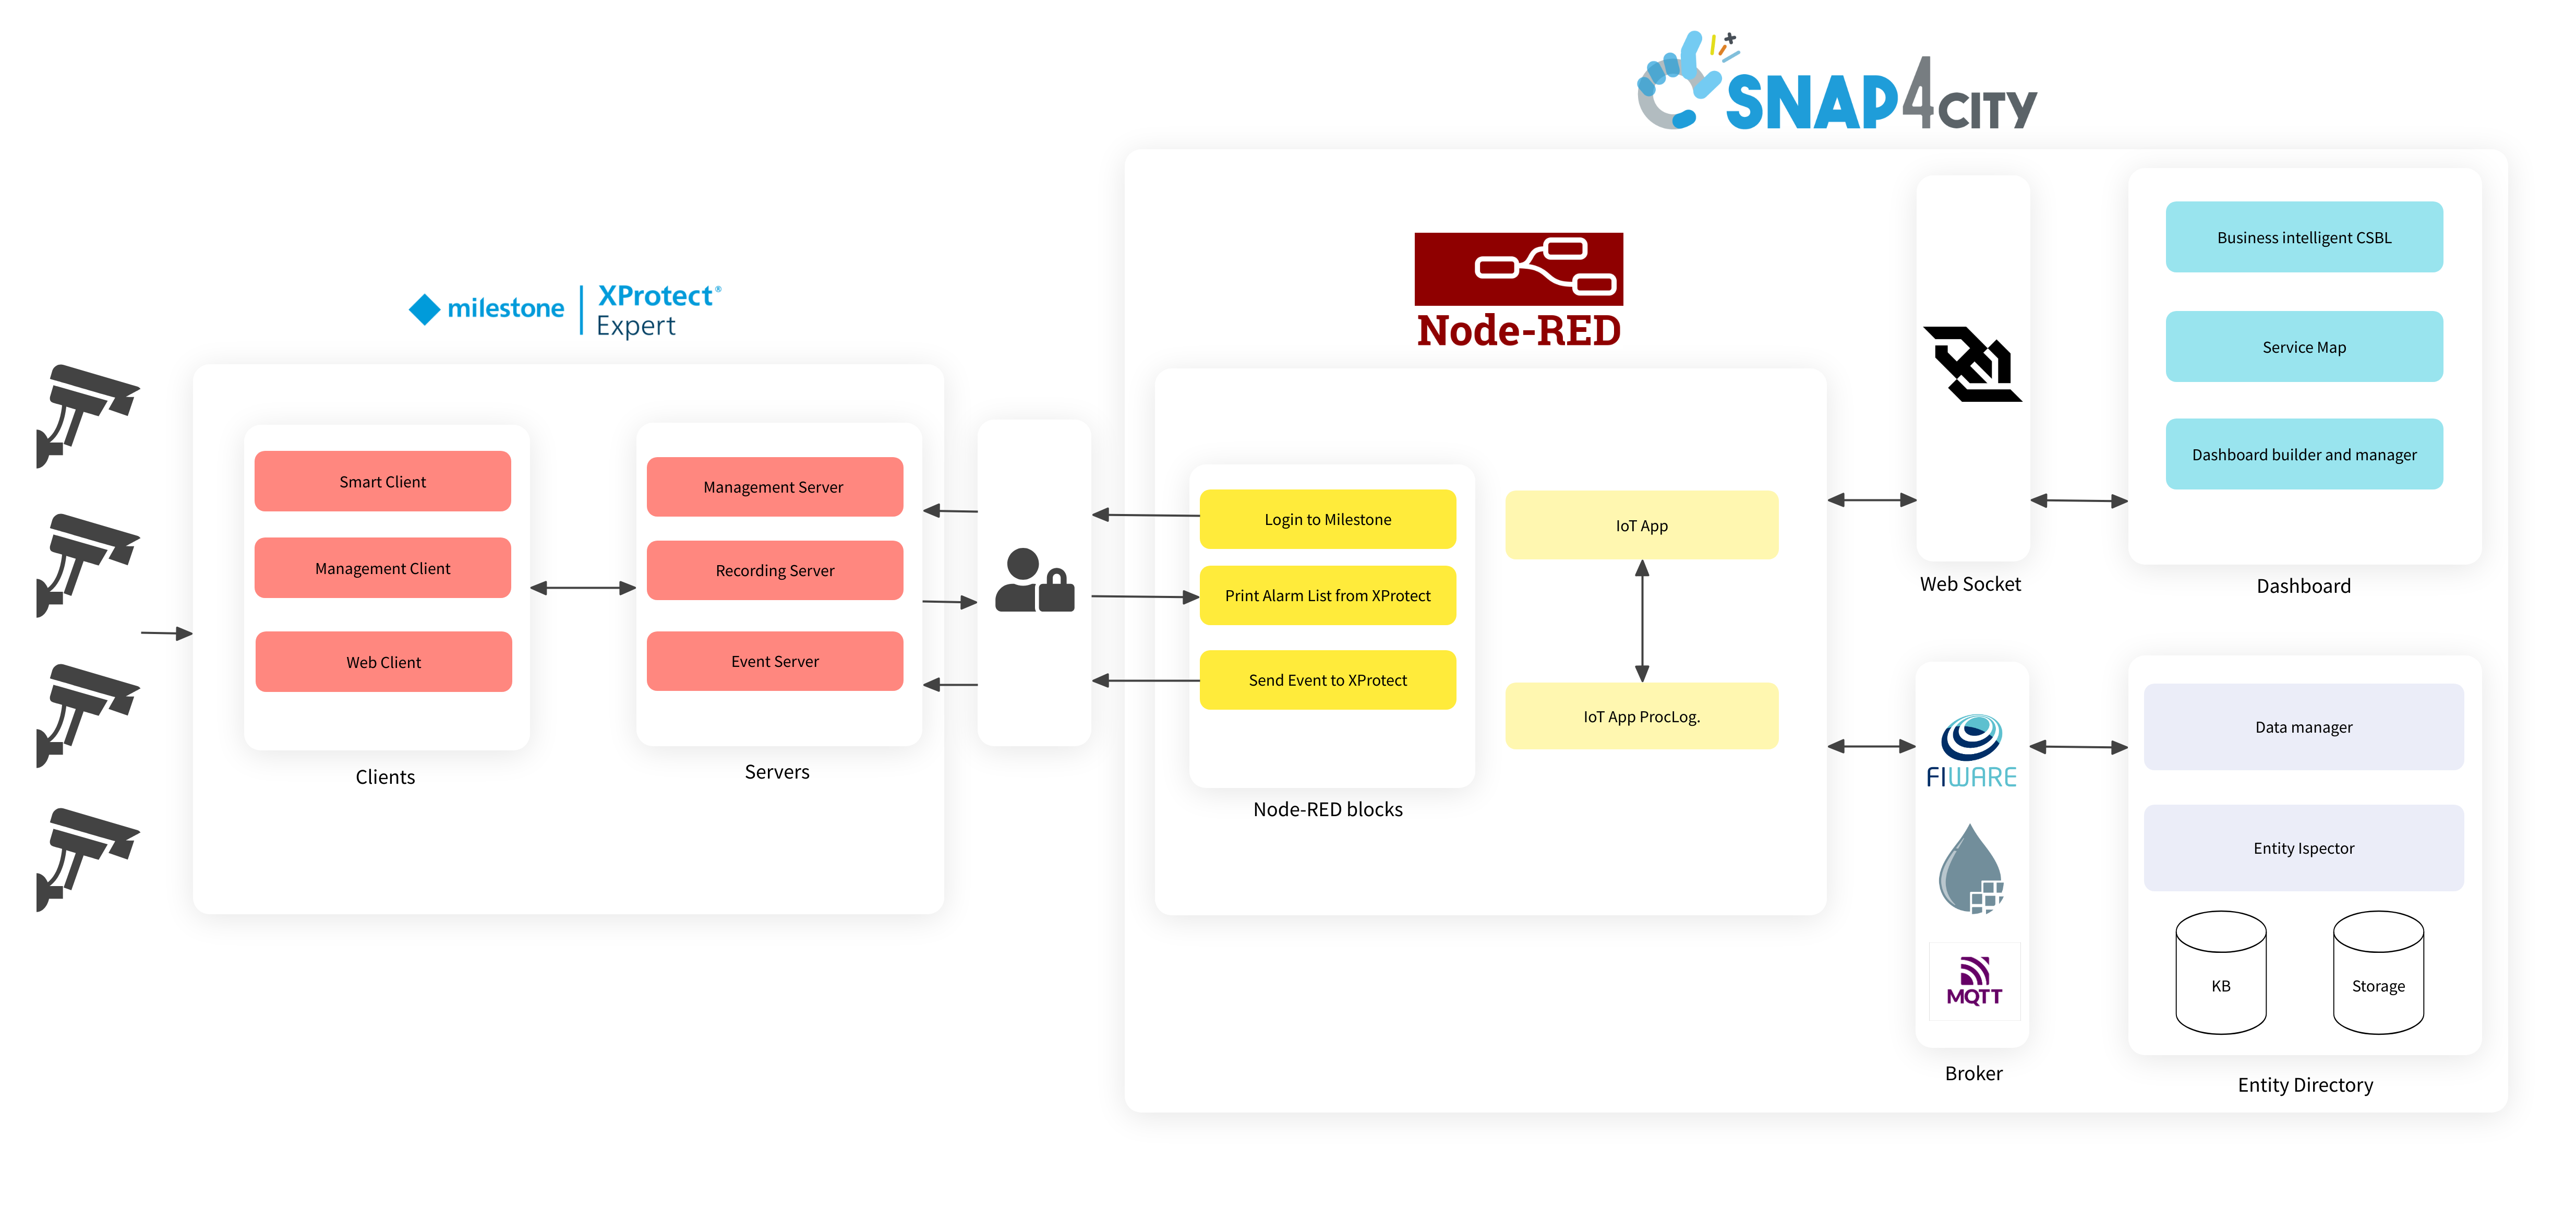
\includegraphics[width = 1\textwidth]{img/arch_final_HQ.png}
    \caption{\textit{Architettura dell'integrazione}}
    \label{archgen}
\end{figure}
\noindent
Il primo elemento è il VMS, che si compone di una parte client e una server. Insieme gestiscono il monitoraggio dei video, la registrazione e la creazione di notifiche.
Il secondo elemento è l’integrazione realizzata tramite Node-RED, che funge da middleware per orchestrare lo scambio di dati tra il VMS e Snap4City implementando flussi specifici per autenticarsi al sistema Milestone, ricevere ed inviare eventi.
La terza componente è rappresentata dalla piattaforma Snap4City, che fornisce strumenti avanzati per l’analisi e la visualizzazione dei dati. Attraverso dashboard interattive e l’integrazione con protocolli Internet of Things (IoT), Snap4City consente agli operatori di monitorare eventi, configurare allarmi e analizzare dati storici. La comunicazione con Node-RED avviene tramite WebSocket per quanto riguarda le dashboard, mentre i dati vengono gestiti e archiviati mediante moduli dedicati, come il data manager e l’entity directory che comunicano con i flussi attraverso un broker basato su FIWARE.

\section{Snap4City} \label{snap4}
Snap4City è una piattaforma IoT e Smart City \cite{snap} progettata per fornire vari servizi
per la gestione e l'analisi dei dati provenienti dall'infrastruttura della città intelligenti, inclusi
sensori, fotocamere e altri dispositivi.
La piattaforma mette a disposizione più di 190 microservizi, gestiti tramite nodi per l’ambiente di
programmazione Node-RED \cite{nodered}, utilizzati come supporto nella gestione delle città intelligenti e a tal
proposito si è scelto di sviluppare una libreria ad hoc per la realizzazione di questa
integrazione.
\begin{figure}[H]
    \centering
    
\includegraphics[width = 0.7\linewidth]{img/logo.png}
\end{figure}


\section{Modelli}

Su Snap4City, i modelli rappresentano una struttura essenziale per la gestione dei dati provenienti dai sensori, consentendo la creazione di dispositivi virtuali, detti device, che ne replicano il comportamento. Attraverso i modelli è possibile standardizzare la configurazione dei sensori, facilitando l'integrazione di diverse tipologie di dispositivi all'interno dell'ecosistema Snap4City. Per ogni tipologia di sensore, viene creato un modello specifico che ne definisce i parametri principali e le modalità di interazione con il sistema.
I principali aspetti configurabili all'interno di un modello includono:

\begin{itemize}
    \item \textbf{Informazioni generali}: comprendono il nome del modello, la descrizione del dispositivo e il nome del produttore.
    \item \textbf{IoT Broker}: funge da intermediario tra il dispositivo e il sistema Snap4City. Il suo scopo è interfacciarsi con i dati prodotti dai dispositivi e renderli accessibili alle applicazioni che ne necessitano.
    \item \textbf{Attributi statici}: sono informazioni che rimangono costanti nel tempo, come la natura e la sottonatura del dispositivo, che ne definiscono il contesto e la destinazione.
    \item \textbf{Attributi dinamici}: sono valori che possono variare nel tempo, come la temperatura, l'umidità o altri dati generati dai device.
\end{itemize}
I modelli sono stati utilizzati per configurare telecamere termiche e gestire eventi. Inoltre, i modelli possono essere estesi per includere eventi specifici, come alert o notifiche, basati su soglie impostate sui valori dinamici dei sensori. Questo approccio consente una gestione flessibile e scalabile dei dispositivi all'interno della piattaforma.

\section{Device}

Un device rappresenta digitalmente entità che vanno dai sensori fisici, come le telecamere termiche, a strutture più astratte, come le heatmap o gli eventi.
Le telecamere sono modellate come device virtuali all'interno della piattaforma, dove vengono registrati i dati rilevati in tempo reale. Questi dispositivi virtuali vengono creati automaticamente a partire dai modelli definiti, utilizzando i flussi Node-RED. Durante la creazione del device, è necessario configurare attributi statici e dinamici che permettono alla piattaforma di gestire correttamente i dati in arrivo.\\ 
Un altro aspetto cruciale riguarda la gestione degli eventi provenienti dal VMS, per questo i device sono progettati per ricevere, gestire ed inviare i dati degli eventi. I dati vengono poi salvati all'interno della piattaforma, creando uno storico utile per monitorare trend e rispondere a situazioni di emergenza.

\section{Milestone Xprotect}
Milestone XProtect è un VMS che offre un'architettura modulare consentendo la gestione centralizzata di infrastrutture di videosorveglianza in contesti di piccole, medie e grandi dimensioni. XProtect supporta l'acquisizione, la registrazione, l'analisi di video e l'integrazione con altri sistemi di sicurezza o piattaforme IoT come Snap4City. Questo può apportare significativi vantaggi nell'ambito delle smart city, migliorando la sicurezza urbana, il coordinamento e la risposta a incidenti facilitando l'analisi in tempo reale di dati visivi.

\subsection{Requisiti tecnici}
Milestone offre diverse versioni della sua piattaforma per soddisfare esigenze differenti a seconda delle proprie necessità \cite{xprotect-version}.
Questa sezione descrive i requisiti tecnici necessari per l'installazione del VMS, compatibile esclusivamente con ambienti Windows e Windows Server. Prima di selezionare la versione più adatta è stato utile consultare la pagina ufficiale di Milestone \cite{requirements}. Qui sono riportati dettagli specifici, incluse le versioni supportate di Microsoft SQL Server \cite{SQLserver} e .NET Framework \cite{.NET}, insieme ai requisiti minimi hardware.
Per il progetto è stata selezionata la versione Expert, che presenta caratteristiche avanzate come una distribuzione multi-server e il supporto per un numero illimitato di dispositivi IP per ogni server di registrazione. Queste funzionalità risultano particolarmente utili e in linea con l'approccio distribuito della piattaforma Snap4City, con cui il sistema dovrà interfacciarsi. In figura \ref{req} sono presenti le specifiche relative alla versione scelta.

\begin{figure}[H]
    \centering
    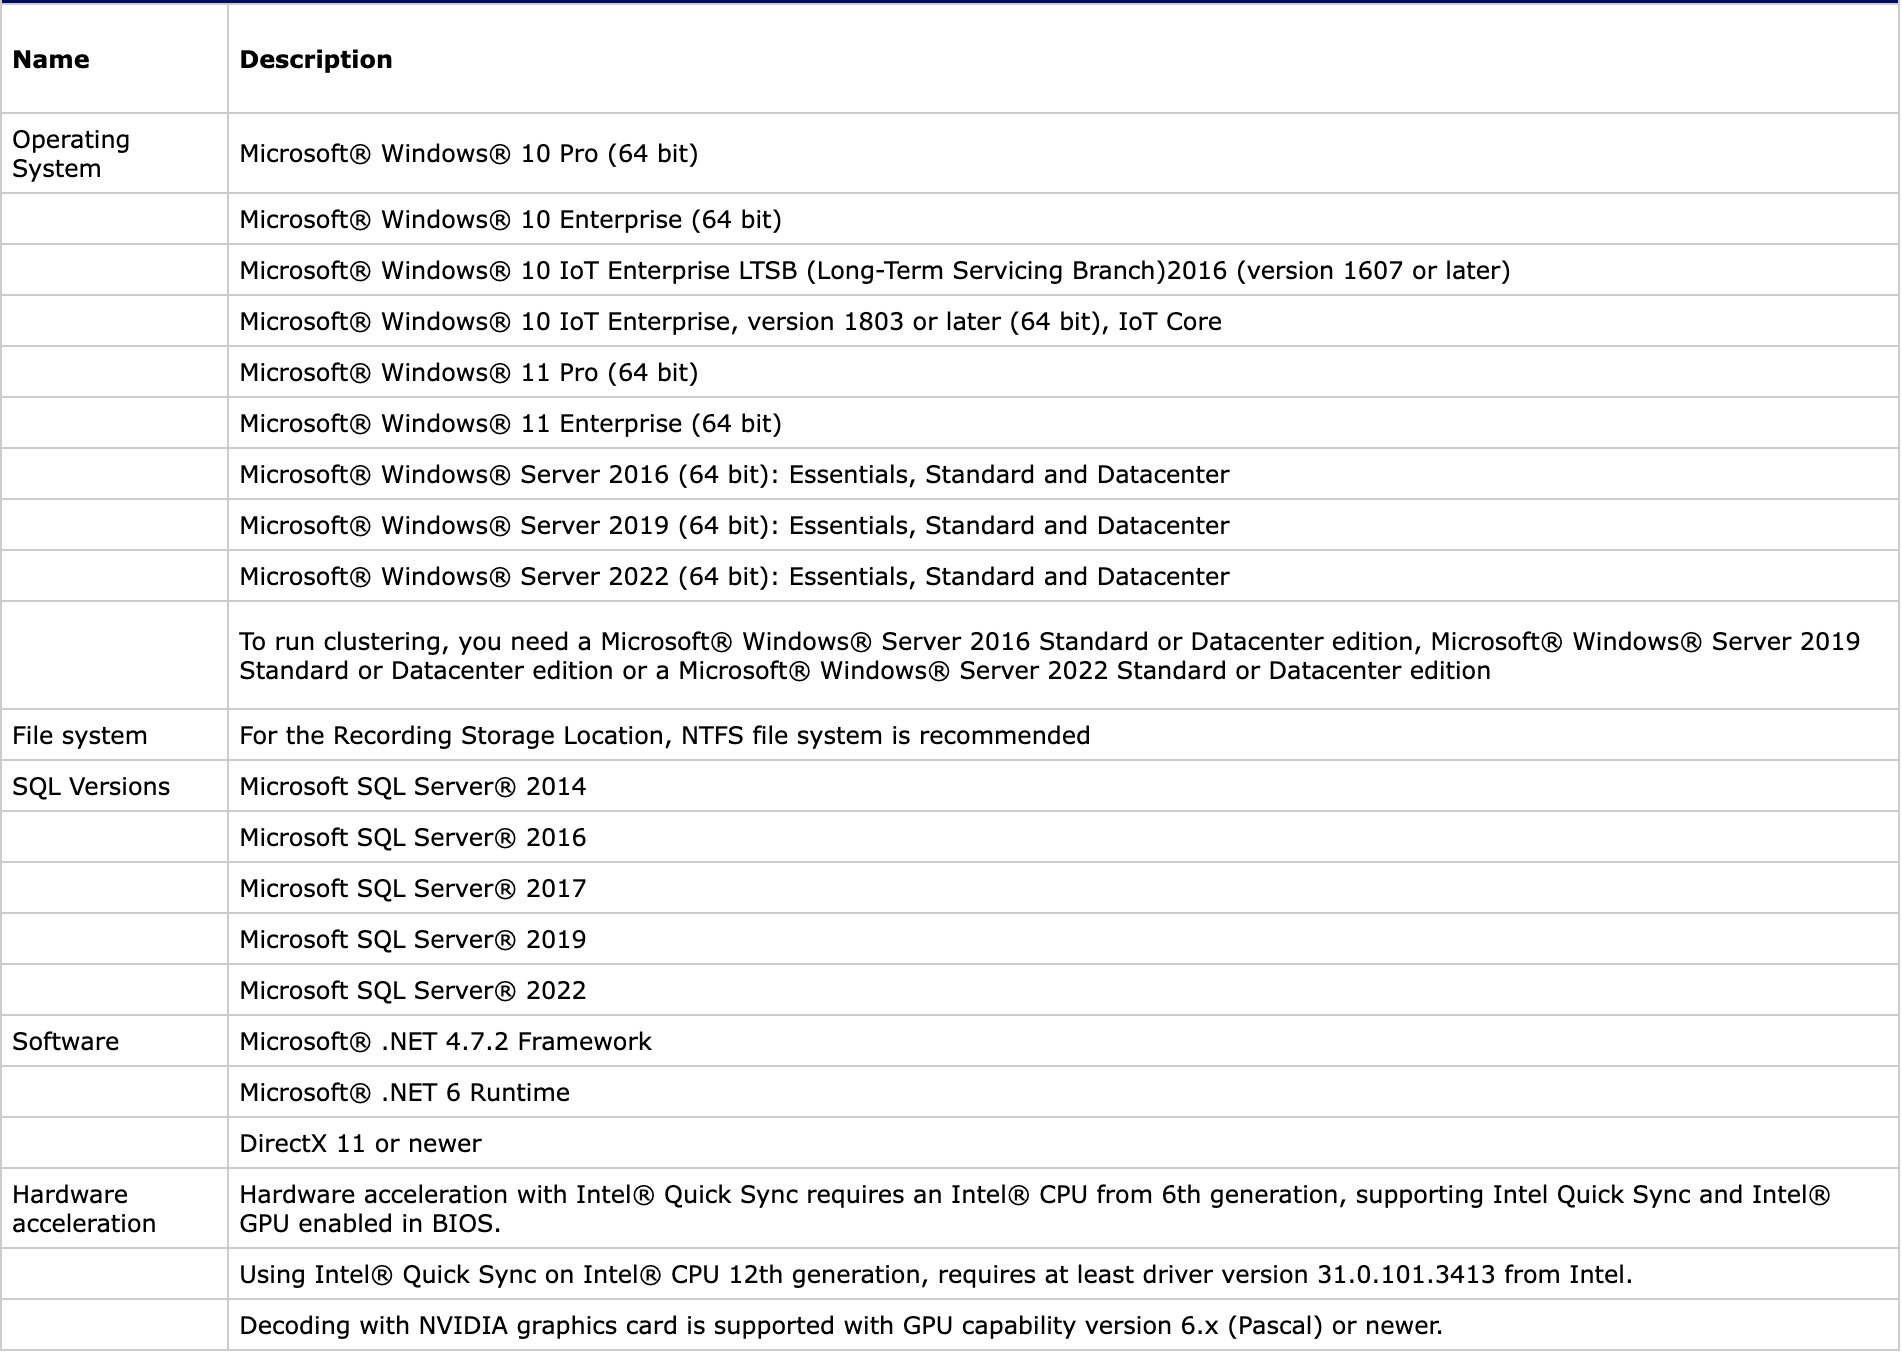
\includegraphics[width=1\linewidth]{img/requirements.png}
    \caption{\textit{Requisiti hardware e software relativi alla versione Expert}}
    \label{req}
\end{figure}

\subsection{Management Server}
Il Management Server rappresenta il cuore dell'architettura XProtect e gestisce la configurazione del sistema, ogni modifica infatti, come l'aggiunta di nuove telecamere o l'aggiornamento delle impostazioni, avviene tramite il Management Server. Questo server memorizza la configurazione del sistema in un database SQL Server, che può essere installato localmente sullo stesso server o su un server SQL dedicato all'interno della rete. Per le installazioni di grandi dimensioni o distribuite, il sistema può supportare un'architettura federata, dove più server collaborano per migliorare le prestazioni e garantire ridondanza.
Il Management Server non solo gestisce le configurazioni ma funge anche da punto centrale di autenticazione per gli utenti, coordinando l'accesso alle risorse video e audio. Tutti i client, sia locali che remoti, si autenticano prima sul Management Server e successivamente accedono ai Recording Server per visualizzare i video registrati.

\subsection{Recording Server}
Il Recording Server è responsabile della comunicazione con le telecamere. Ogni flusso video o audio acquisito viene archiviato in un database multimediale ad alte prestazioni, appositamente progettato per ottimizzare la memorizzazione e il recupero di dati video. Questo database supporta funzionalità avanzate come l'archiviazione su più livelli, la firma digitale dei video e la crittografia delle registrazioni, assicurando l'integrità e la sicurezza dei dati.
Il Recording Server non solo memorizza le registrazioni, ma le rende accessibili ai vari client del sistema, sia per la visualizzazione live sia per la riproduzione. Il server supporta inoltre la gestione delle telecamere in modalità multicast per ottimizzare la trasmissione dei dati in reti complesse. Inoltre, in caso di interruzioni di rete o malfunzionamenti, Milestone offre un server di registrazione failover \cite{failover}, da configurare per garantire continuità operativa.

\subsection{Event Server}
L’Event Server gestisce eventi, allarmi e integrazioni con plugin di terze parti. Consolidando tutti gli eventi del sistema in un unico punto, facilita le integrazioni con software esterni tramite il Milestone Integration Platform (MIP) \cite{mipdoc}. È responsabile della gestione di allarmi, mappe, e dell'archiviazione dei dati relativi agli eventi in un database SQL condiviso con il Management Server.
L'Event Server permette anche l'invio di messaggi in tempo reale tra client e server e consente l'automazione di azioni tramite regole basate su eventi. In caso di attivazione di un evento ad esempio, un movimento rilevato da una telecamera,  può attivare allarmi o notifiche specifiche agli operatori.

\subsection{Management Client}
Il Management Client è l'interfaccia principale per amministrare il sistema XProtect. Comunicando con i server descritti in precedenza consente la configurazione centralizzata e l’amministrazione quotidiana del sistema, offrendo strumenti per la gestione dei dispositivi, dei server e degli utenti. Il Management Client fornisce anche un controllo granulare sulle autorizzazioni degli utenti, permettendo agli amministratori di definire profili utente personalizzati.
Una delle caratteristiche chiave del Management Client è la gestione delle regole, che permette agli amministratori di creare flussi di lavoro automatizzati in risposta a determinati eventi.

\subsection{Smart Client}
Lo Smart Client \cite{smartclient} è un'applicazione desktop progettata per fornire agli operatori un controllo intuitivo sui sistemi di sicurezza. Oltre a visualizzare i flussi video live, si possono eseguire ricerche avanzate sui video registrati, gestire allarmi e visualizzare metadati generati da analitiche video o altre fonti.
Lo Smart Client è personalizzabile infatti l'interfaccia può essere adattata in base al livello di competenza degli utenti e alle loro specifiche responsabilità. L'accesso ai dati e alle funzionalità del sistema può essere limitato in base ai ruoli assegnati dall’amministratore, garantendo una gestione sicura e centralizzata.
L'integrazione con applicazioni esterne tramite il MIP Software Development Kit (SDK) \cite{sdk} permette di estendere le funzionalità del client con analisi video avanzate e integrazioni di sistemi di sicurezza aziendali.

\subsection{Web Client}
Il Web Client \cite{webclient} è un’applicazione web che permette agli utenti di accedere al sistema XProtect da qualsiasi browser, senza la necessità di installare software aggiuntivo. Offre funzionalità base di monitoraggio video, come la visualizzazione live e la riproduzione delle registrazioni, nonché la possibilità di esportare clip video e stamparne i fotogrammi.
Nonostante le sue funzionalità semplificate rispetto allo Smart Client, è uno strumento efficace per utenti remoti che necessitano di un accesso rapido e sicuro alle funzioni di base del VMS. La possibilità di accedere al sistema da qualsiasi dispositivo connesso a Internet lo rende una scelta ideale per il monitoraggio mobile e per il personale che opera da remoto.

\section{Milestone Integration Platform e MIP SDK}
La Milestone Integration Platform (MIP) è una piattaforma software tramite la quale si
possono implementare diversi tipi di integrazione tra i prodotti Milestone e altre applicazioni o
dispositivi di terze parti in svariati scenari quali l’analisi audio e video, il controllo degli
accessi, la gestione di eventi e allarmi, l’automazione degli edifici e il controllo del VMS.
Questo viene sviluppato grazie al MIP SDK con cui è possibile realizzare
operazioni che vanno da quelle più semplici e dirette, a quelle più
complesse.
In figura \ref{ex} di seguito viene illustrata l’architettura della piattaforma con riferimento alla comunicazione tra le
diverse componenti e le varie funzionalità rese disponibili da Milestone.

\begin{figure}[H]
    \centering
    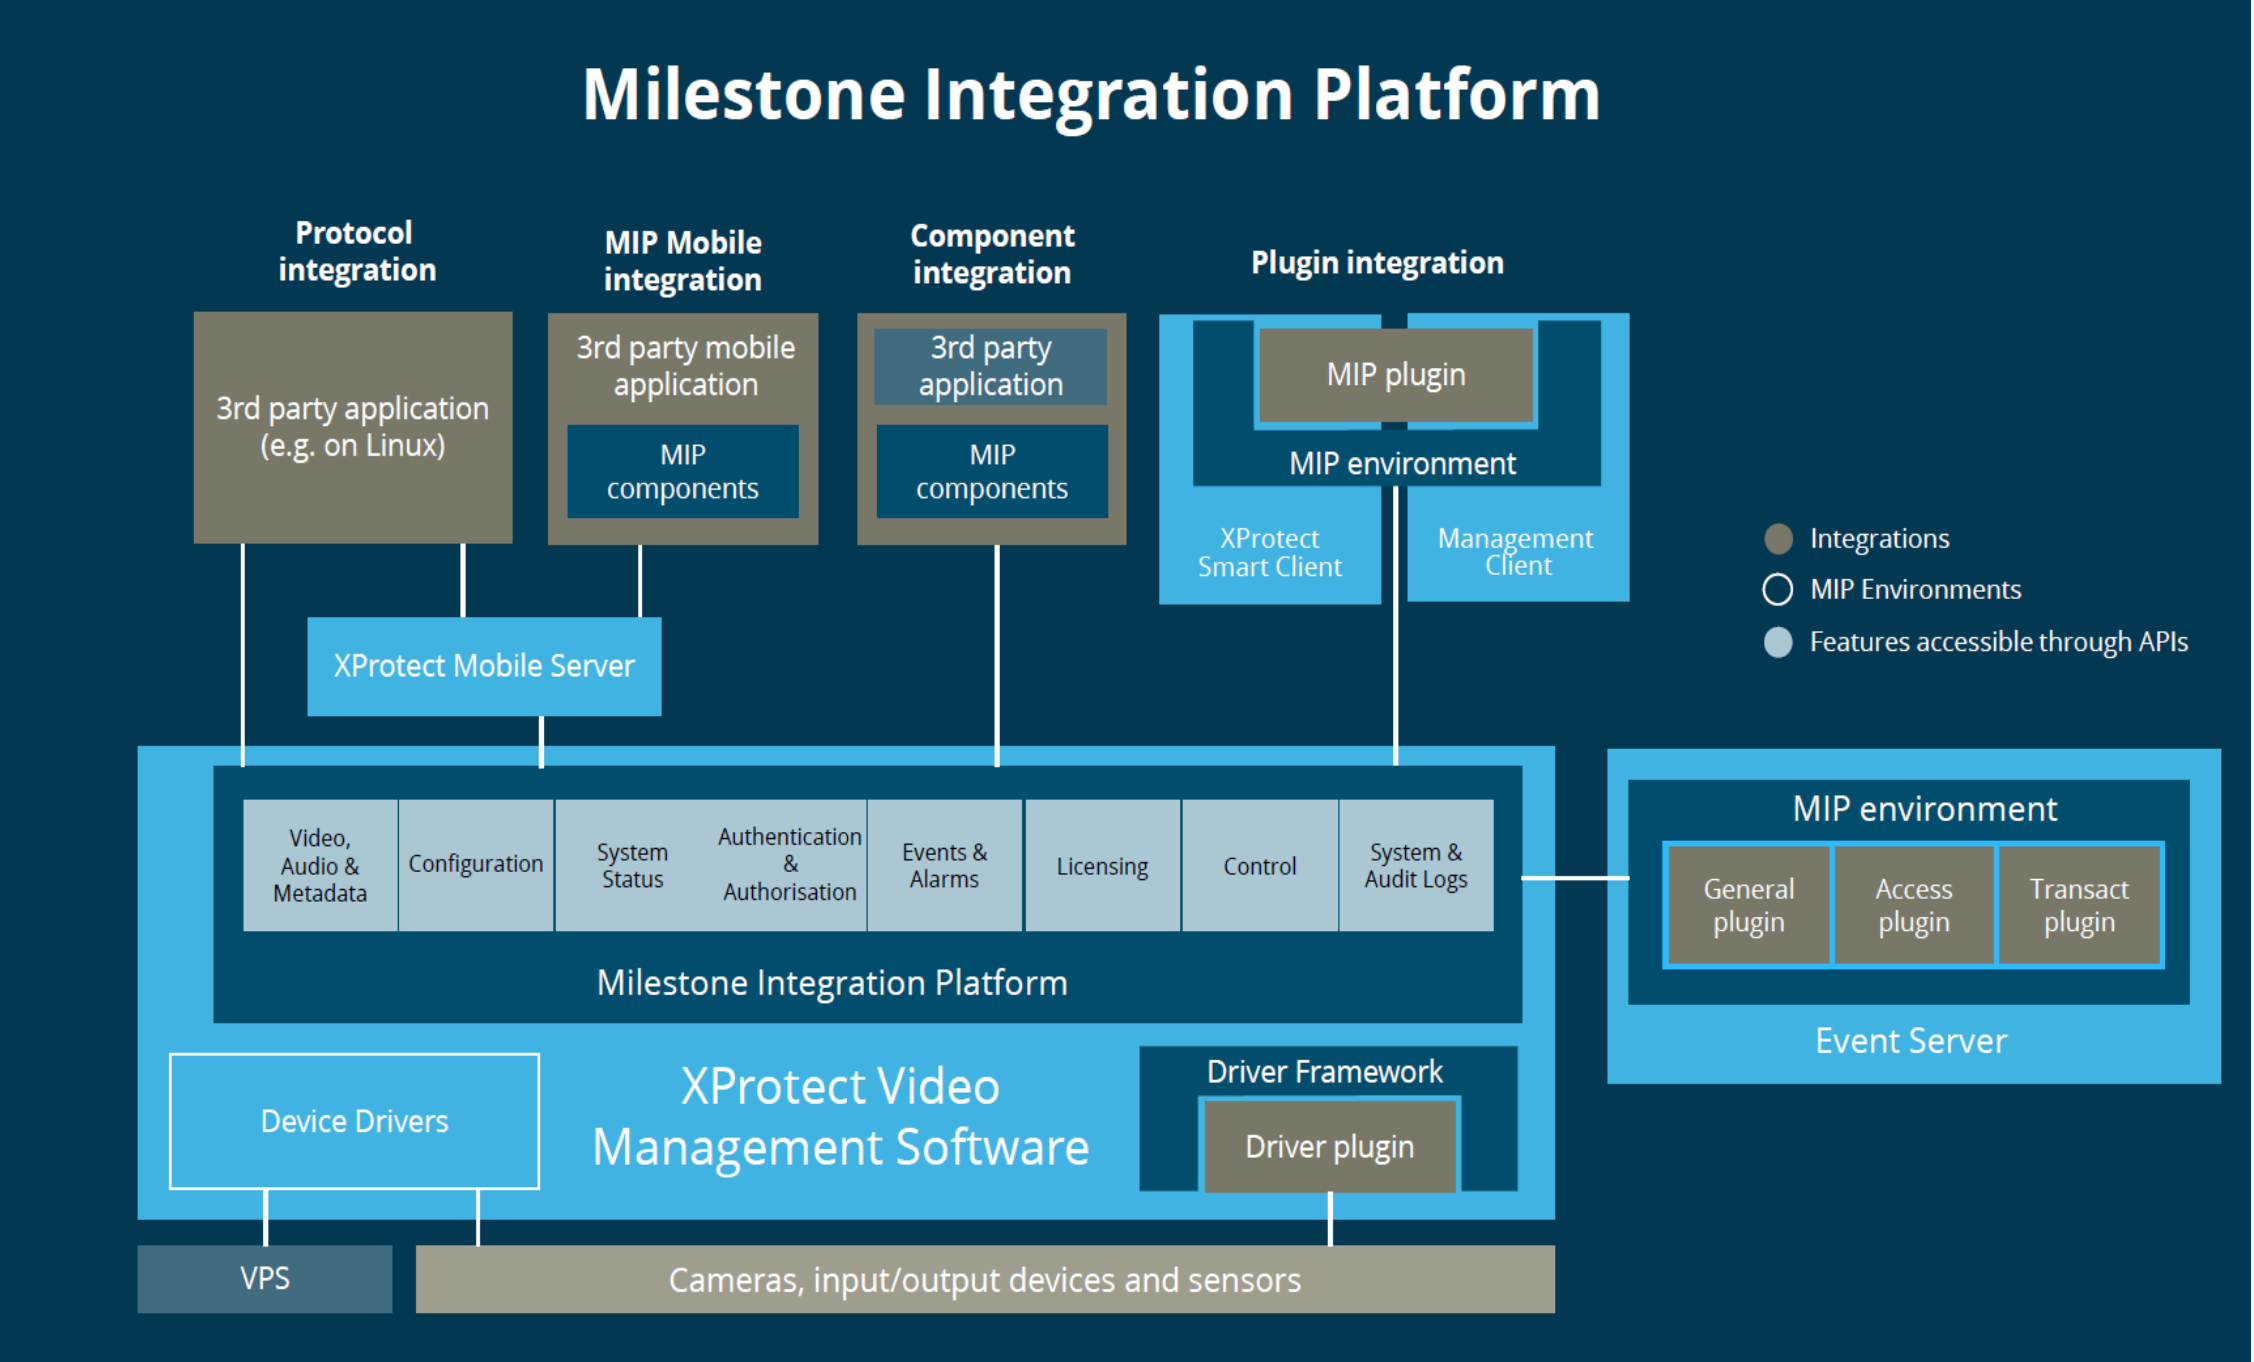
\includegraphics[width=1\linewidth]{img/1.png}
    \caption{\textit{Architettura di Milestone Integration Platform}}
    \label{ex}
\end{figure}
 
\subsection{Possibili soluzioni e scelte adottate}
Un punto chiave consiste nella scelta del giusto approccio di integrazione che diventa
fondamentale per raggiungere l’obiettivo prefissato, vengono dunque elencati i tre tipi di
integrazione messi a disposizione, con i relativi vantaggi e svantaggi:
\begin{itemize}
    \item \textbf{Component integration:} tramite questa integrazione è possibile utilizzare i componenti MIP con i quali si può interagire con il VMS e i server, senza il bisogno di installare i loro prodotti. Questo approccio è quindi il più adatto quando si vuole realizzare una propria applicazione, che ad esempio accede ai video o condivide dati con il VMS, senza la necessità della presenza di applicazioni XProtect. I contro sono dati dall’obbligo di utilizzare un linguaggio che supporta .NET e dal fatto che l’applicazione deve essere necessariamente sviluppata per piattaforma Windows.
    \item \textbf{Plugin integration:} un plug-in può essere eseguito nei vari prodotti Milestone che supportano MIP
    consentendone un utilizzo multiplo, a fronte di un’unica implementazione. L’approccio tramite plug-in offre quindi la possibilità di sviluppare funzionalità senza dover
    costruire un ambiente di hosting e il vantaggio di avere un’integrazione diretta all'interno degli ambienti client e server di Milestone attraverso la piattaforma MIP. Anche in questo caso lo svantaggio è che richiede un ambiente .NET per lo sviluppo.
    \item \textbf{Protocol integration:} utilizzando questo approccio si può accedere alla configurazione del VMS Milestone, ottenere video, inviare comandi e scaricare eventi dai server. Questo anche se l’applicazione da integrare non è eseguita su un sistema operativo Microsoft Windows, oppure è stata sviluppata in un linguaggio che non supporta .NET, con lo svantaggio di avere una più alta complessità nell’implementazione di funzionalità rispetto alle due integrazioni elencate in precedenza che sono invece più dirette.
\end{itemize}
Considerando pro e contro dei diversi approcci e le due piattaforme che dovranno essere
integrate si è scelto di utilizzare la protocol integration. Innanzitutto perché permette lo sviluppo di un’applicazione senza vincoli di sistema operativo o di linguaggio di programmazione, e in secondo luogo perché le funzionalità da implementare per questo progetto non richiedono
ulteriori servizi offerti dalle altre due integrazioni rispetto a questa.

\section{Node-RED}
Node-RED è un ambiente di sviluppo basato su flussi, progettato per la connessione e l'integrazione di dispositivi, API e servizi online in modo visuale e intuitivo. \'E particolarmente utilizzato per facilitare l'integrazione di sistemi IoT, permettendo agli utenti di creare flussi di dati e processi automatizzati senza la necessità di scrivere codice complesso.
Grazie alla sua interfaccia, è possibile creare flussi personalizzati che automatizzano la raccolta, l'elaborazione e l'invio di dati, integrando diversi dispositivi IoT e sistemi esterni.
\begin{figure}[H]
    \centering
    
\includegraphics[width=0.7\linewidth]{img/noderedlogo.png}
\end{figure}

\section{Sviluppo nuovi blocchi}
Come anticipato nella sezione \ref{snap4} è stata realizzata una libreria Node-RED, chiamata \textit{node-red-contrib-snap4city-milestone} \cite{noderedmilestone}, che permette l’interazione con il VMS tramite una protocol integration con la quale è possibile fare il login e, una volta ottenuti i
permessi, inviare o ricevere eventi. Di seguito vengono descritti la struttura e la logica dei vari nodi implementati per le diverse operazioni.

\subsection{Login}\label{login} \'E un nodo è fondamentale per l’integrazione perché attraverso questo si
ottengono i permessi per comunicare con il VMS. Infatti, dopo aver inserito hostname, nome utente e password registrati sulla piattaforma vengono restituiti
2 token, uno per le chiamate alle REST API \cite{RestAPIdoc} e uno per le SOAP API \cite{SoapAPIdoc}, entrambi necessari per
le operazioni di invio/ricezione eventi.
Nelle figure \ref{2} e \ref{3} sono riportate le interfacce del nodo su Node-RED e quella di
configurazione per inserire i dati richiesti per l’operazione.

\begin{figure}[H]
    \centering
    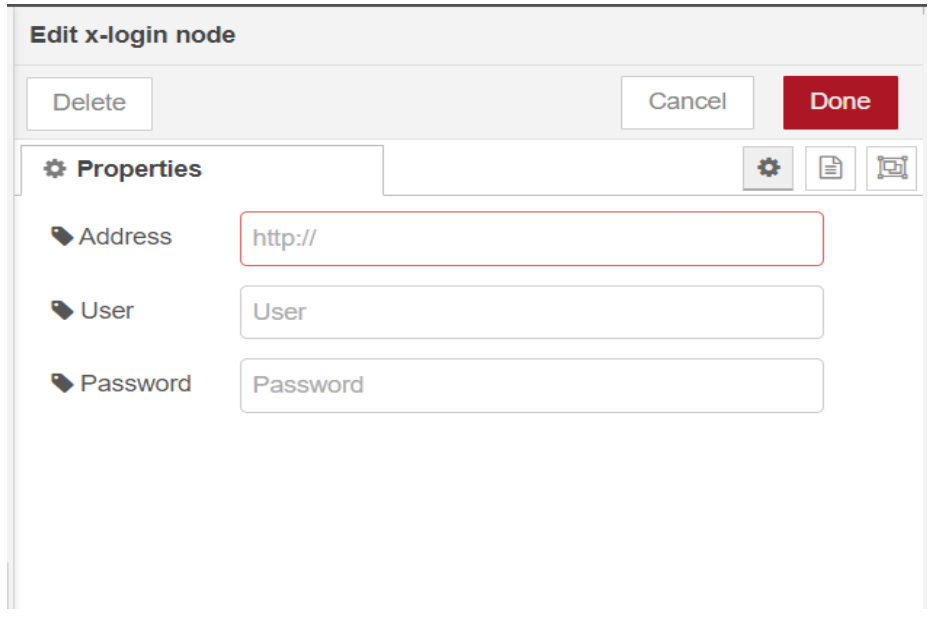
\includegraphics[width=0.5\linewidth]{img/2.png}
    \caption{\textit{Configurazione del nodo Login}}
    \label{2}
\end{figure}

\begin{figure}[H]
    \centering
    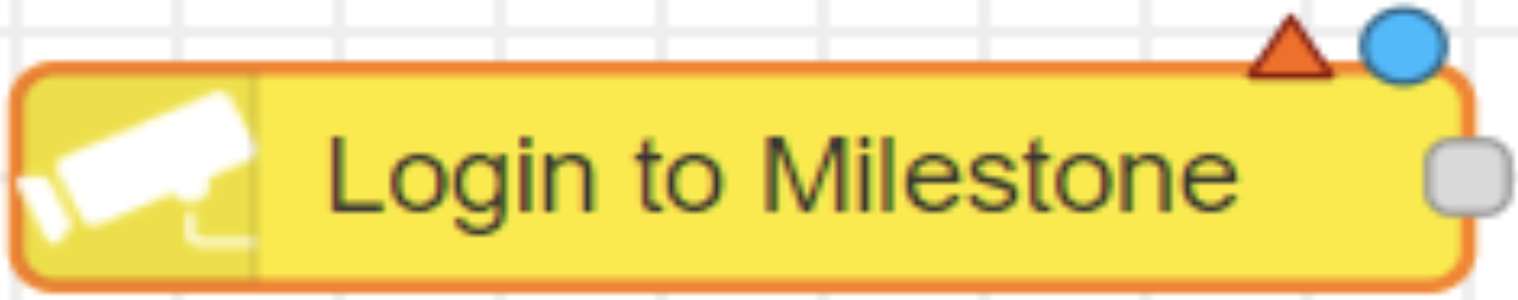
\includegraphics[width=0.5\linewidth]{img/3.png}
    \caption{\textit{Interfaccia del nodo Login}}
    \label{3}
\end{figure}
\noindent La logica per ottenere i token di accesso è implementata attraverso le due funzioni principali \textit{getTokenREST} e \textit{getTokenSOAP}.
La prima invia una richiesta HTTP POST ad un endpoint specifico del server IDP con le credenziali fornite e restituisce un token di accesso per le REST API.
La seconda invece invia una richiesta SOAP al server di gestione tramite un payload XML specifico con le credenziali incluse nell'intestazione \textit{Authorization} in formato \textit{Basic Auth} e restituisce un token di accesso per le SOAP API.
Nei codici \ref{lst:getTokenREST} e \ref{lst:getTokenSOAP} viene mostrata l'implementazione delle due funzioni.
\begin{figure}[H]
    \centering
    \lstinputlisting[
        style=customJS,
        caption={Funzione \textit{getTokenREST}},
        label={lst:getTokenREST}
    ]{code/getTokenREST.js}
    \vspace{1em}
    \lstinputlisting[
        style=customJS,
        caption={Funzione \textit{getTokenSOAP}},
        label={lst:getTokenSOAP}
    ]{code/getTokenSOAP.js}
\end{figure}



\subsection{Invio eventi al VMS}\label{sendevent}
Grazie a questo nodo è possibile comunicare con l’event server di Milestone inviando un evento da Node-RED il quale attiva un evento analitico, salvato sul VMS, che al momento dell’attivazione mostra un allarme all’operatore che lo sta
utilizzando con le informazioni relative all’evento inviato. In figura \ref{4} è presente uno
schema logico fornito da Milestone nella documentazione \cite{eventdoc} che riassume il funzionamento, fornendo due approcci diversi.

\begin{figure}[H]
    \centering
    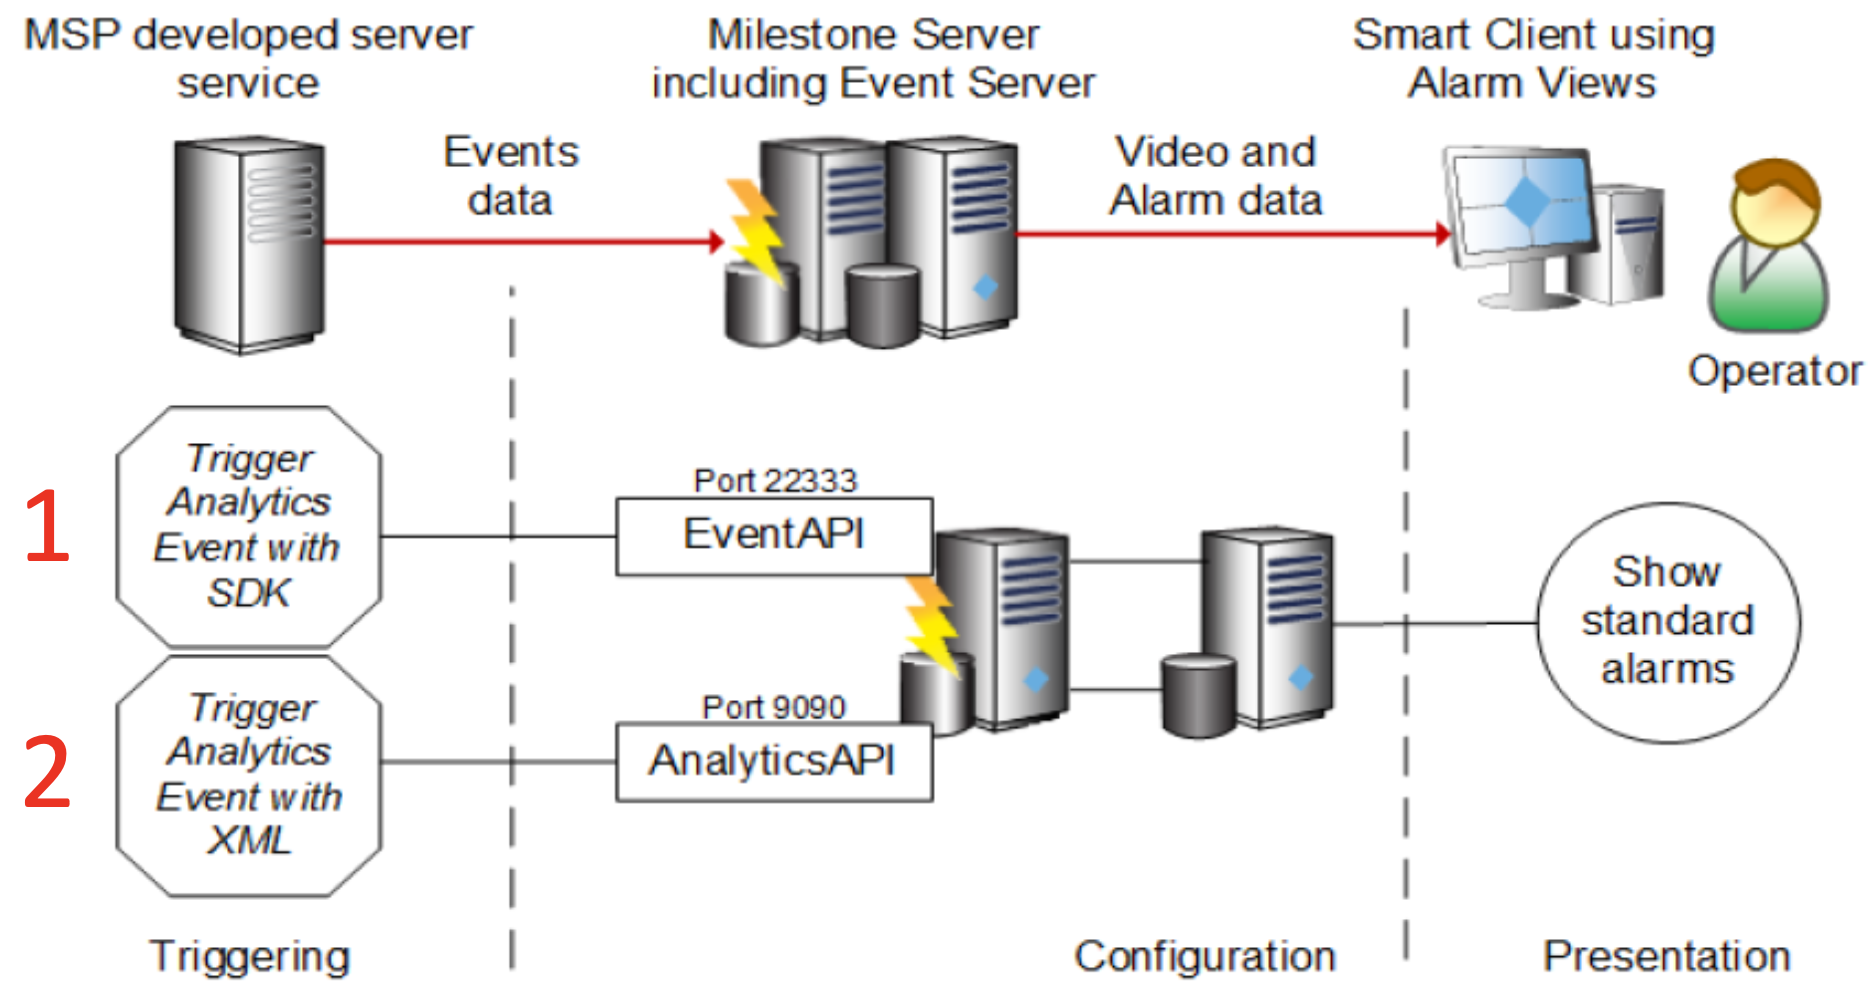
\includegraphics[width=1\linewidth]{img/4.png}
    \caption{\textit{Schema logico di invio eventi al VMS}}
    \label{4}
\end{figure}
\noindent
Si è scelto di usare l’approccio tramite chiamate SOAP, quindi con l’invio di documento
XML (2), perché tra le due è la soluzione che non necessita di un ambiente .NET. Il documento XML viene creato grazie ai dati ricevuti in ingresso al nodo cioè il nome
dell’evento, l’ID della telecamera, l’hostname del VMS, la porta che espone gli eventi analitici e una
breve descrizione, come possiamo vedere nella figura \ref{5} in seguito.
\begin{figure}[H]
    \centering
    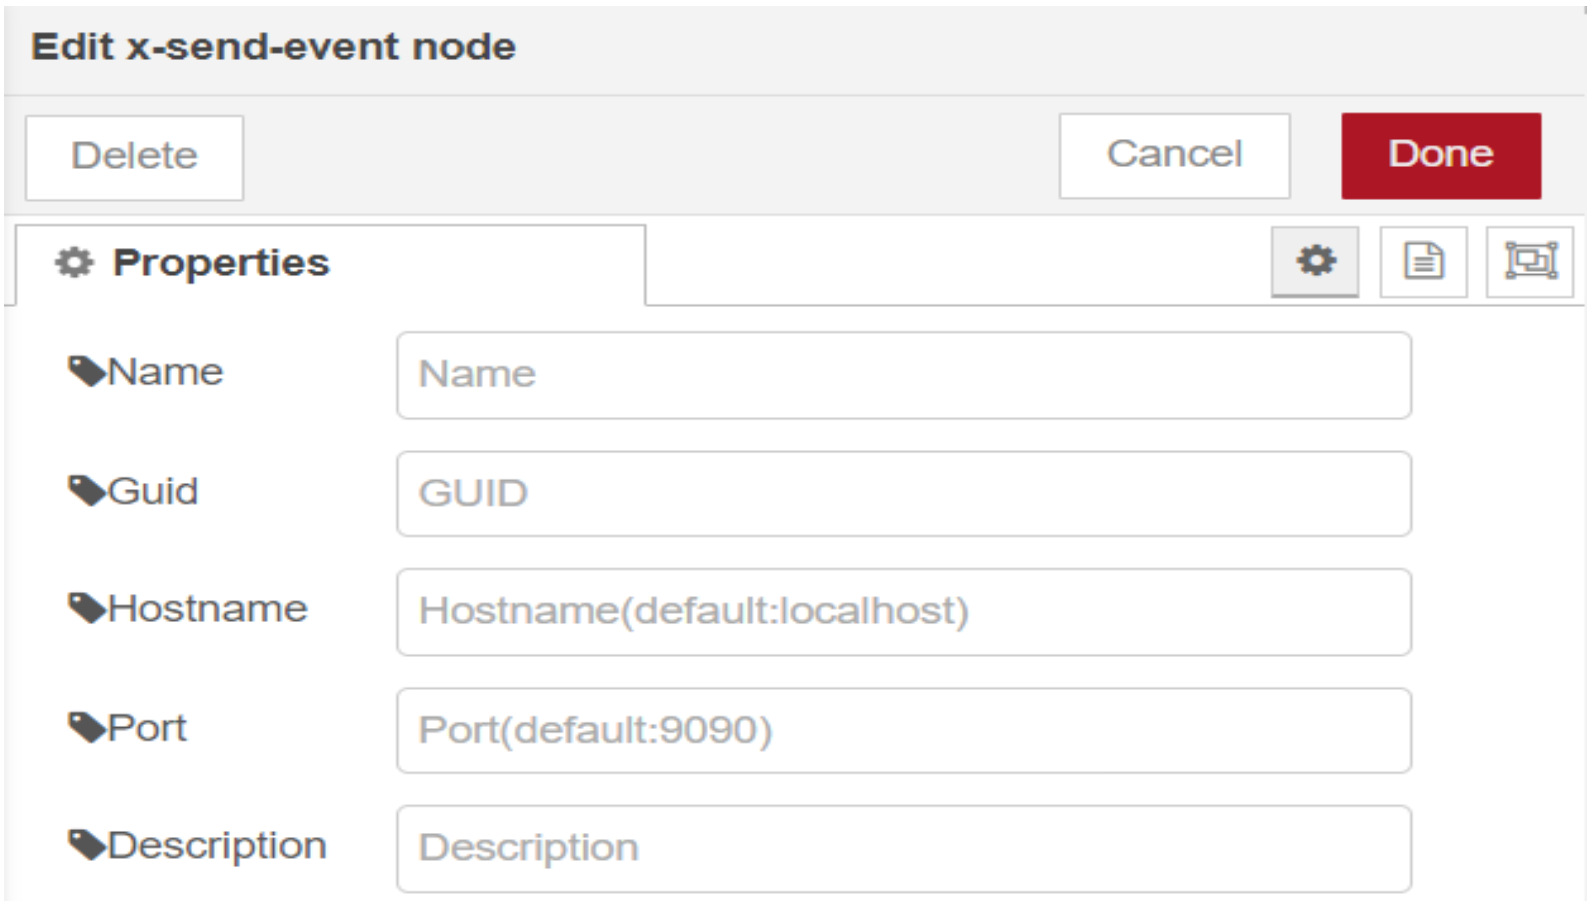
\includegraphics[width=0.5\linewidth]{img/6.png}
    \caption{\textit{Configurazione del nodo di invio eventi}}
    \label{5}
\end{figure}

\begin{figure}[H]
    \centering
    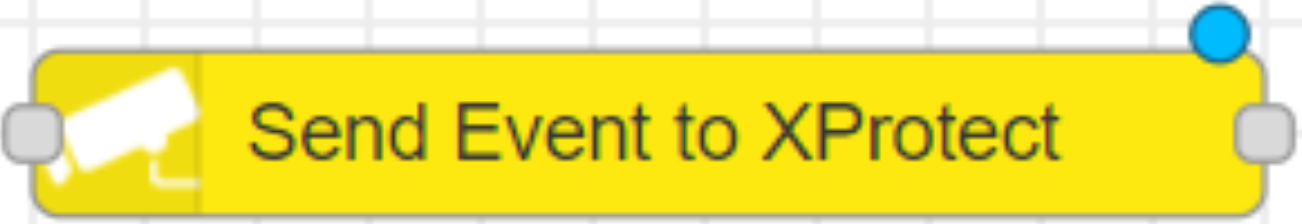
\includegraphics[width=0.5\linewidth]{img/5.png}
    \caption{\textit{Interfaccia del nodo di invio eventi}}
    \label{6}
\end{figure}
\noindent
La funzione principale di questo nodo è \textit{sendXML}, riportata in Codice \ref{lst:sendXML}, che si occupa di inviare un evento analitico in formato XML. Per prima cosa, la funzione utilizza il metodo \textit{getAllEvents} dell'oggetto \textit{Gateway} per recuperare l'elenco completo degli eventi disponibili. Successivamente, verifica se un evento con il nome specificato è già presente. Se l'evento esiste, la funzione genera un messaggio XML utilizzando la funzione \textit{eventXML} e invia una richiesta POST all'URL fornito. In caso contrario, restituisce un messaggio di errore indicando che l'evento richiesto non esiste. Inoltre, la funzione gestisce eventuali errori di connessione, restituendo un messaggio dettagliato che descrive il problema riscontrato. Il risultato della richiesta, sia esso un successo o un errore, viene restituito come valore della funzione.

\begin{figure}[H]
    \centering
    \lstinputlisting[
        style=customJS,
        caption={Funzione \textit{sendXML}},
        label={lst:sendXML}
    ]{code/sendXML.js}
\end{figure} 
\noindent
È importante ricordare che per un utilizzo corretto di questo nodo è necessario configurare il VMS e quindi attivare la porta degli eventi analitici, creare l’evento analitico
che verrà attivato all’arrivo dell’evento e definire l’allarme mostrato all’operatore.

\subsection{Ricezione eventi dal VMS}\label{receivevent}
L’implementazione di questo nodo è fondamentale per ricevere gli eventi attivati nel VMS indipendentemente dalla sorgente che l’ha generato.
Dal punto di vista implementativo è simile al nodo di invio evento, quindi comunicazione tramite event server con chiamate SOAP e documento XML, con la differenza che la porta
di accesso diventa quella di tutti gli eventi e non solo quella degli eventi analitici.
Per il corretto funzionamento del nodo è necessario verificare quale sia la porta degli eventi all’interno del VMS e se è attiva. Anche in questo caso il documento XML è creato con i dati ricevuti in ingresso al nodo quindi l’hostname del VMS, la porta degli eventi, il numero massimo di eventi che si
vogliono ricevere, l’ordine con cui si vogliono visualizzare (crescente o decrescente) e il
target a cui applicare tale ordinamento. Nelle figure \ref{7} e \ref{8} si vede come configurare questi parametri e l'interfaccia su node-RED.

\begin{figure}[H]
    \centering
    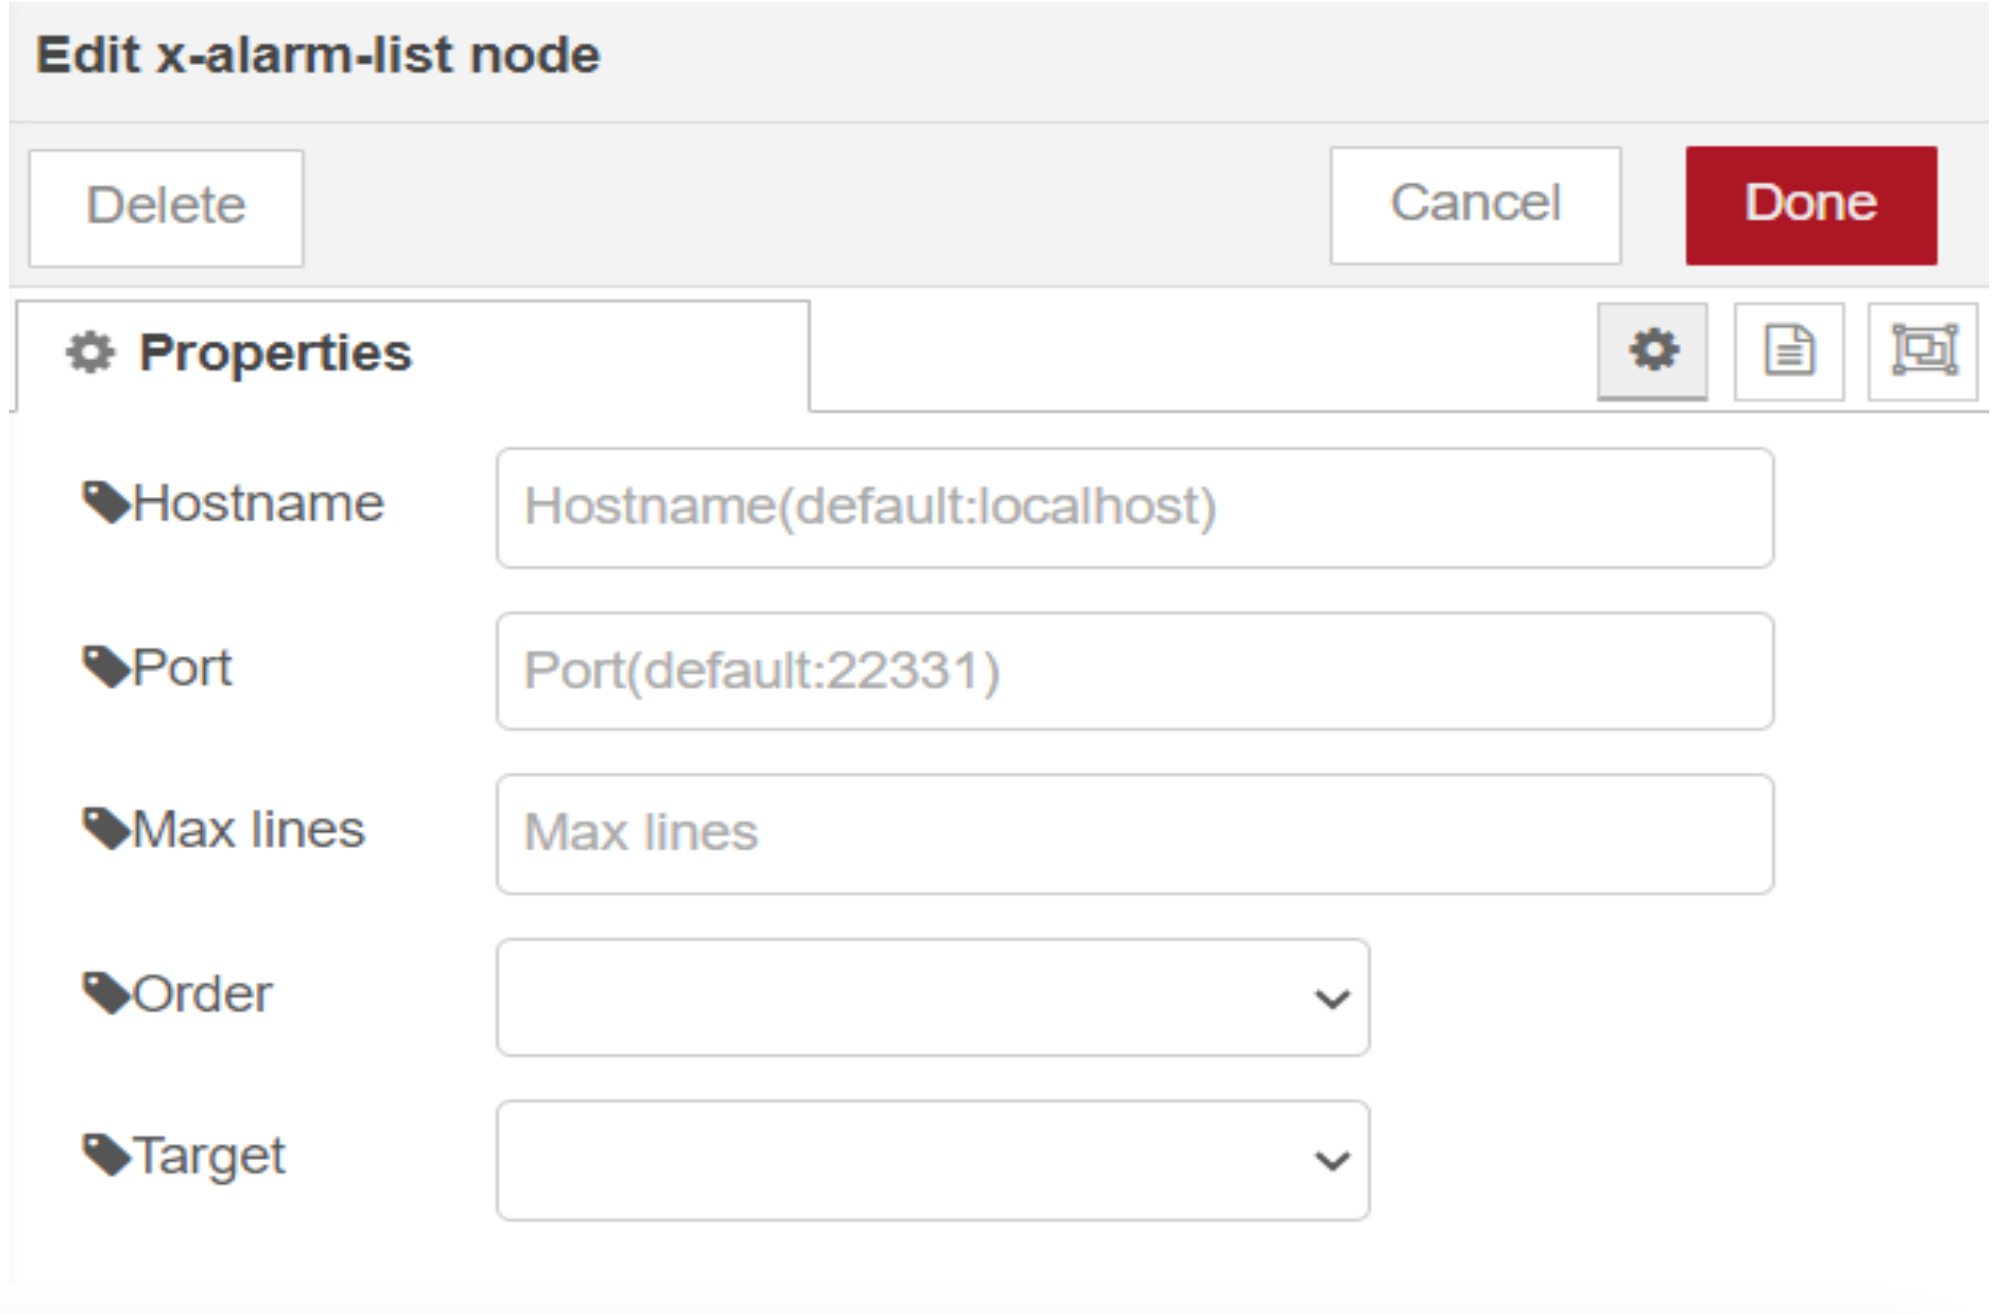
\includegraphics[width=0.5\linewidth]{img/8.png}
    \caption{\textit{Configurazione del nodo di ricezione eventi}}
    \label{7}
\end{figure}

\begin{figure}[H]
    \centering
    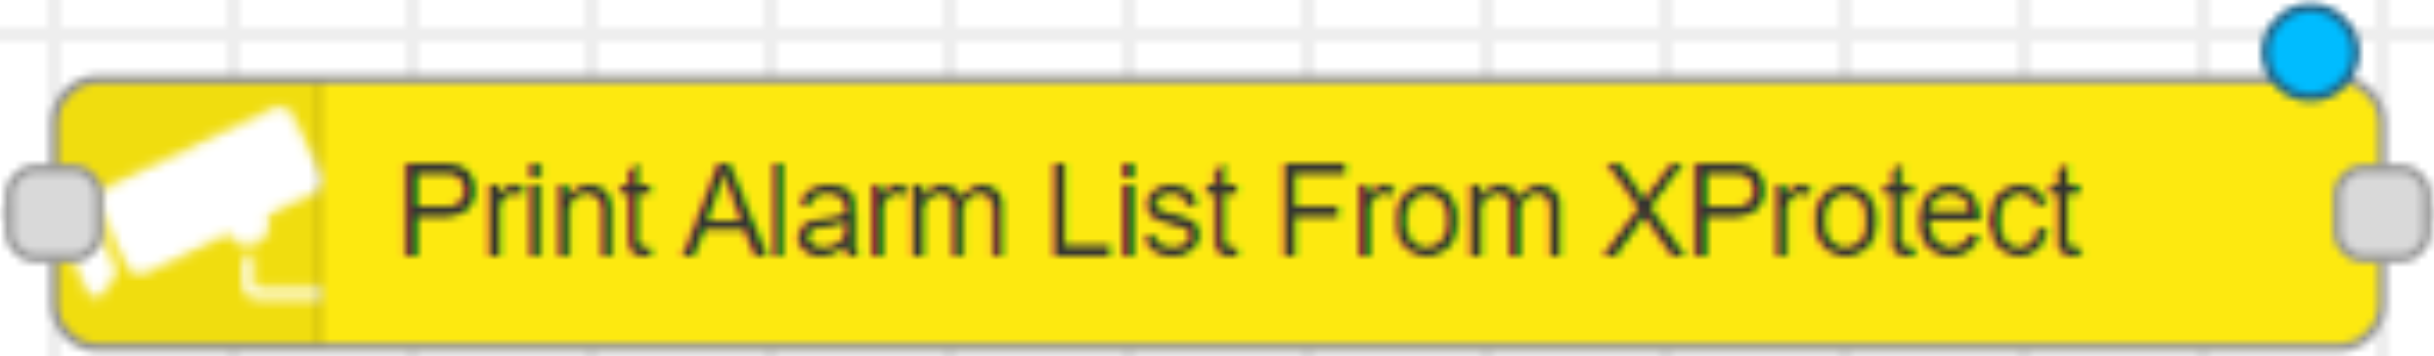
\includegraphics[width=0.5\linewidth]{img/7.png}
    \caption{\textit{Interfaccia del nodo di ricezione eventi}}
    \label{8}
\end{figure}
\noindent
Come visto per gli altri nodi, la funzione chiave in questo caso è \textit{getAlarmList} mostrata nel Codice \ref{lst:getAlarmList} che è usata per recuperare la lista degli allarmi dal VMS tramite una comunicazione SOAP. All'inizio viene chiamata \textit{getAlarmLines} per ottenere i dati sugli allarmi, utilizzando i parametri descritti in precedenza. Se la risposta non è un oggetto valido, viene trattata come un errore, e il messaggio di errore viene separato per restituire una descrizione. In caso contrario, la risposta XML viene convertita in JSON e se la risposta è valida, la funzione esamina il contenuto degli allarmi e restituisce un elenco strutturato di oggetti, con ogni allarme rappresentato come una mappa di nome e informazioni associate. Se si verifica un errore, la funzione fornisce un oggetto contenente l'errore e la relativa descrizione.

\begin{figure}[H]
    \centering
    \lstinputlisting[
        style=customJS,
        caption={Funzione \textit{getAlarmList}},
        label={lst:getAlarmList}
    ]{code/getAlarmList.js}
\end{figure} 

\chapter{PROGETTAZIONE}
In questo capitolo vengono descritti i modelli progettati per consentire l'integrazione tra Snap4City e VMS. Questa si basa sulla creazione di modelli specifici per la gestione di dati provenienti da telecamere termiche e per il monitoraggio degli eventi. Ogni modello definisce una struttura funzionale che standardizza la configurazione e il flusso di dati, facilitando il collegamento e l’interazione tra i dispositivi IoT e il VMS. \\ Il modello \textit{MilestoneCamera} è stato concepito per identificare e localizzare le telecamere termiche all'interno della rete, mentre i modelli \textit{AlertMilestone} e \textit{AlertListener} supportano la gestione degli eventi e degli allarmi. Questi ultimi sono fondamentali per rilevare condizioni di interesse e inviare notifiche tempestive, rispondendo in modo dinamico ai dati provenienti dai sensori video. \\ Attraverso una progettazione mirata, ciascun modello offre un contributo specifico all’architettura complessiva, consentendo una gestione efficace e scalabile dei dispositivi e degli eventi all'interno dell'infrastruttura della smart city.
\section{MilestoneCamera}
Questo modello fornisce le informazioni essenziali per localizzare e identificare una telecamera specifica all’interno della rete.
Nella configurazione di una telecamera termica, i parametri principali includono:
\begin{itemize}
\item\textbf{ipAddress}: rappresenta l'indirizzo IP della telecamera e costituisce l'elemento centrale per il collegamento diretto alla risorsa fisica, consentendo l'accesso remoto a immagini e video in tempo reale.

\item\textbf{CamId}: è un identificatore univoco assegnato a ciascuna telecamera all’interno del sistema che permette di distinguere i flussi video e di tracciare dati ed eventi provenienti da specifiche telecamere.

\item\textbf{Description}: fornisce una breve descrizione della telecamera, utile per indicare informazioni di contesto e riferimenti intuitivi per gli operatori o per il sistema automatizzato (ad esempio, "Entrata Nord" o "Parcheggio 1").

\item\textbf{dateObserved}: indica la data e l’ora in cui è stata effettuata l’ultima osservazione o rilevazione della telecamera, garantendo che i dati recuperati siano aggiornati e sincronizzati.

In figura \ref{9} viene illustrata l'interfaccia di creazione del modello su Snap4City con i vari parametri d'interesse.

\end{itemize}
\begin{figure}[H]
    \centering
    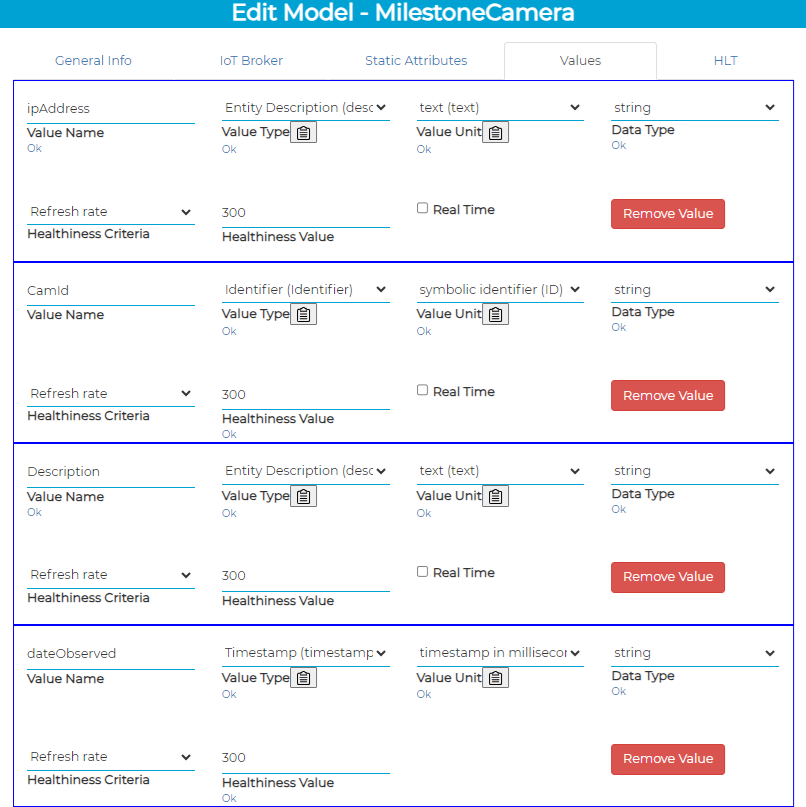
\includegraphics[width=1\linewidth]{img/CamModel3.png}
    \caption{\textit{ Attributi dinamici del modello MilestoneCamera}}
    \label{9}
\end{figure}

\section{AlertMilestone} \label{alertmilestone}
Questo modello è stato progettato per ricevere e gestire eventi generati dal VMS, permettendo a Snap4City di ottenere informazioni dettagliate su situazioni di interesse rilevate dalle telecamere o dagli operatori, e di integrarle nel sistema di monitoraggio della smart city. Il modello, come si vede nelle figure \ref{10}, \ref{11} e \ref{12}, raccoglie una serie di parametri che forniscono un'informazione critica per identificare e contestualizzare l'evento all'interno dell'infrastruttura urbana.
\begin{itemize}
\item\textbf{SourceName}: indica la telecamera o il dispositivo specifico che ha generato l'evento, facilitando la localizzazione della sorgente.
\item\textbf{Position}: rappresenta la posizione del dispositivo, specificando la sua collocazione all'interno della smart city tramite latitudine e longitudine.
\item\textbf{Description}: una breve descrizione dell'evento, utile per fornire una sintesi immediata.
\item\textbf{Status}: rappresenta lo stato dell’evento nel momento della generazione (ad esempio, "nuovo", "in corso" o "risolto").
\item\textbf{Kind}: definisce il tipo di evento, facilitando la categorizzazione per una gestione più ordinata.
\item\textbf{User}: identifica l'utente o l'entità responsabile per la gestione dell'evento, che potrebbe essere una risorsa automatizzata o un operatore umano.
\item\textbf{Severity}: identifica la gravità dell'evento, rendendo possibile un'analisi della priorità.
\item\textbf{People}: registra il numero di persone coinvolte nell'evento, una metrica significativa per il tipo di risposta da attivare.
\item\textbf{Impact}: descrive l'impatto dell'evento, utile per una valutazione preliminare.
\item\textbf{City e Address}: specificano il luogo dell’evento, facilitando l’intervento locale.
\item\textbf{DateObserved}: registra il momento esatto della generazione dell’evento, garantendo una tracciabilità temporale.
\end{itemize}
\begin{figure}[H]
    \centering
    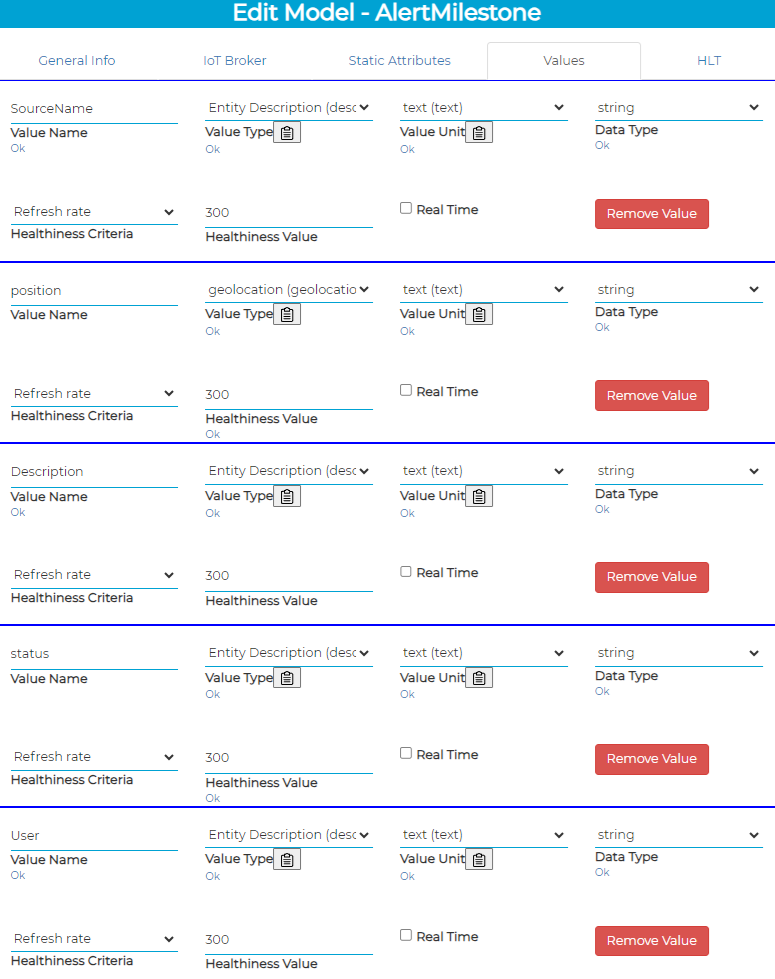
\includegraphics[width=1\linewidth]{img/AlertMilestone3.png}
    \caption{\textit{ Attributi dinamici del modello AlertMilestone(1)}}
    \label{10}
\end{figure}

\begin{figure}[H]
    \centering
    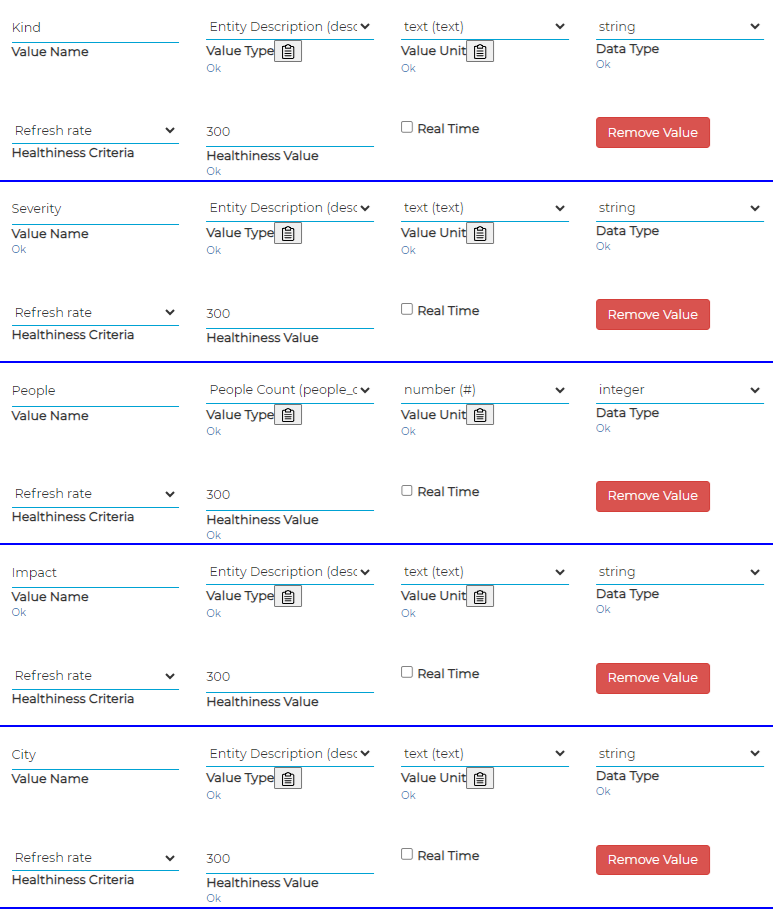
\includegraphics[width=1\linewidth]{img/AlertMilestone4.png}
    \caption{\textit{ Attributi dinamici del modello AlertMilestone(2)}}
    \label{11}
\end{figure}

\begin{figure}[H]
    \centering
    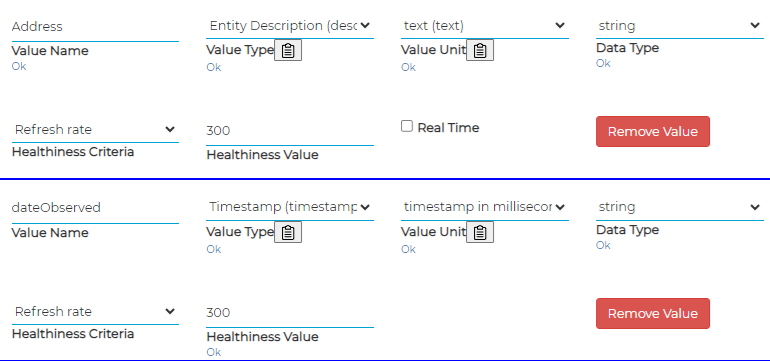
\includegraphics[width=1\linewidth]{img/AlertMilestone5.png}
    \caption{\textit{ Attributi dinamici del modello AlertMilestone(3)}}
    \label{12}
\end{figure}

\section{AlertListener}
Il modello \textit{AlertListener} è stato concepito per inviare eventi dalla piattaforma Snap4City al VMS. Gli eventi generati tramite questo modello possono essere innescati direttamente da una dashboard di Snap4City, offrendo agli operatori uno strumento per segnalare manualmente situazioni rilevanti e trasmetterle al VMS, facilitando un monitoraggio centralizzato. Si riporta di seguito la descrizione solo degli attributi che differiscono dal modello precedente:
\begin{itemize}
\item\textbf{Name}: identifica l’evento generato, consentendo di attribuirgli un’etichetta specifica e facilmente riconoscibile.
\item\textbf{GPS}: fornisce la posizione geografica precisa dell'evento, un'informazione fondamentale per il VMS per correlare l'evento con le risorse vicine.
\end{itemize}
\noindent
L’AlertListener è quindi uno strumento che permette di creare un canale di comunicazione diretto con il VMS, utilizzabile per segnalazioni e richieste di intervento, supportando la gestione reattiva delle situazioni monitorate.
\noindent
Questa differenziazione nei modelli, pur mantenendo una base strutturale comune, garantisce che le due piattaforme siano perfettamente allineate, scambiandosi dati sugli eventi in modo coordinato ma flessibile. La simmetria tra i due modelli permette quindi una gestione bidirezionale degli eventi, assicurando che ogni evento rilevante venga monitorato, registrato e gestito, indipendentemente dalla sua fonte o dalla necessità di intervento.
Nella figura \ref{13} viene mostrata una schermata di Snap4City per visualizzare la lista dei vari device creati in base ai diversi eventi avvenuti all'interno della smart city.
\begin{figure}[H]
    \centering
    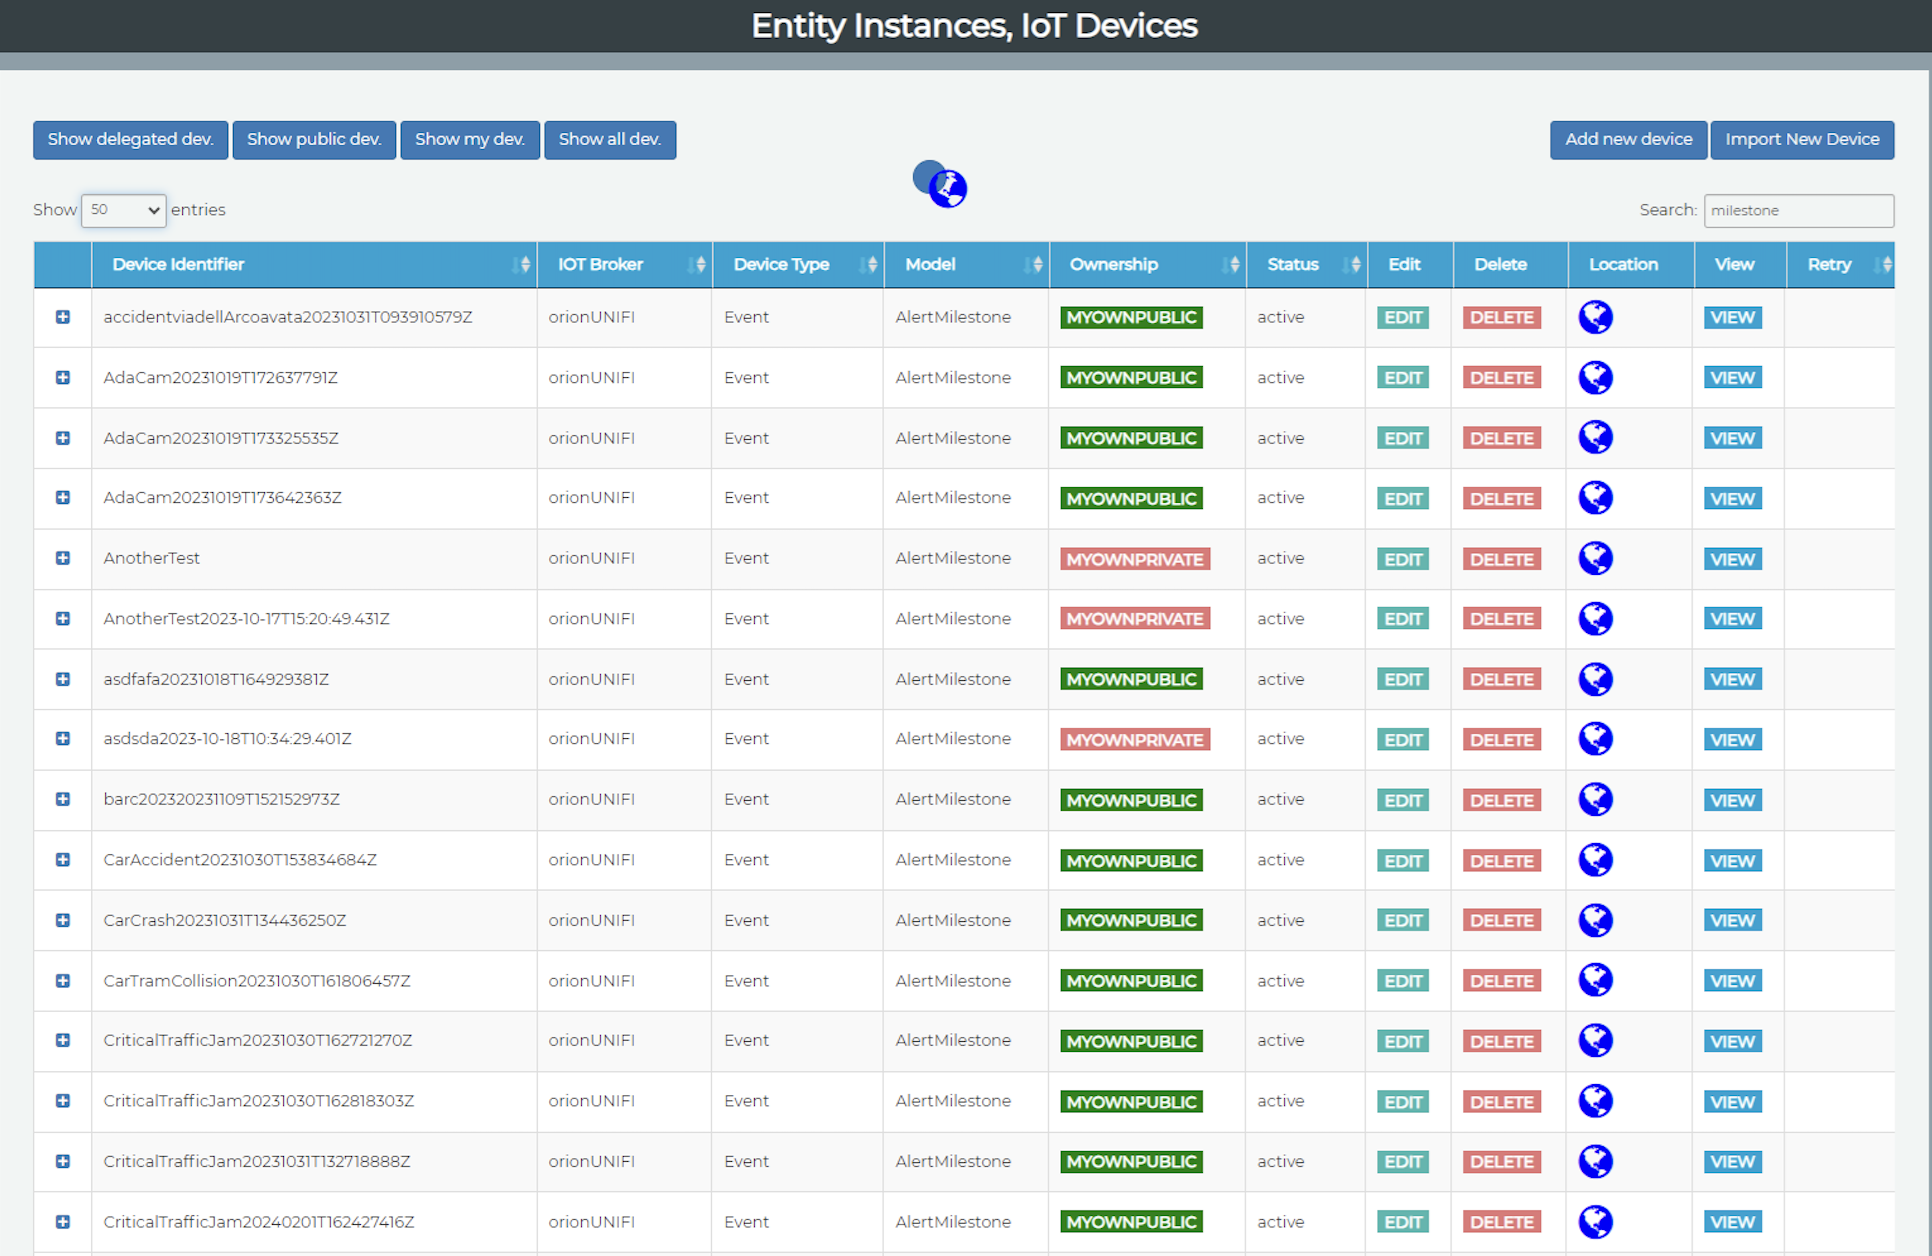
\includegraphics[width=1\linewidth]{img/DeviceListing.png}
    \caption{\textit{ Lista dei device creati}}
    \label{13}
\end{figure}

\chapter{IMPLEMENTAZIONE}
Il presente capitolo illustra i dettagli tecnici e operativi dell'implementazione del sistema progettato per integrare l'infrastruttura IoT di Snap4City con il VMS.
Le sezioni successive si concentrano su tre principali componenti:
\begin{itemize}
      \item \textbf{Flussi Node-RED}: viene analizzato lo sviluppo dei flussi per l'interazione tra i due sistemi, evidenziando come questi permettano di inviare e ricevere eventi generati in tempo reale. I flussi gestiscono inoltre l'autenticazione, l'elaborazione, la trasformazione e l'inoltro dei dati, garantendo una rappresentazione standardizzata degli eventi.
    \item \textbf{Dashboard}: si descrive il ruolo della dashboard come interfaccia principale per la supervisione e l’interazione con gli eventi. Questa sezione approfondisce le funzionalità di visualizzazione dei flussi video delle telecamere e la gestione degli scenari simulati, supportando una risposta operativa rapida ed efficace.
    \item \textbf{VMS}: si dettaglia la configurazione del sistema di gestione video, con particolare attenzione alla configurazione delle telecamere, all'accesso alle immagini in tempo reale e alla gestione di allarmi e notifiche.
\end{itemize}

\section{Flussi Node-RED}
I flussi implementati in Node-RED costituiscono il fulcro dell’integrazione, garantendo uno scambio di dati bidirezionale in tempo reale.
Di seguito sono descritti i due principali flussi sviluppati: il primo dedicato alla creazione di eventi da Snap4City verso il VMS, e il secondo progettato per il monitoraggio degli eventi generati dal VMS e il loro inserimento in Snap4City.

\subsection{Da Snap4city al VMS}
Il primo flusso è stato sviluppato per la creazione e l'invio degli eventi da Snap4City, che tramite una dashboard consente agli operatori di inserire manualmente avvisi e segnalazioni rilevanti direttamente sulla mappa della smartcity specificando i dettagli dell'evento. Come mostrato in figura \ref{14}, questi parametri vengono acquisiti dal flusso Node-RED in ascolto sulla dashboard tramite il  blocco \textit{fiware orion subscribe api v2}. Una volta ricevuto il payload viene formattato per renderlo compatibile al modello AlertMilestone analizzato nella sezione \ref{alertmilestone} e con il blocco \textit{iotdirectory-new-device-from-model} viene creato il device. Il flusso successivamente si occupa di inserire i dati specificati dall'utente che finalizza l'operazione con \textit{fiware orion out api v2}.
L'integrazione tra Node-RED e il VMS avviene attraverso il blocco \textit{Send Event to Xprotect} sviluppato ad hoc e descritto nel capitolo \ref{sendevent}, che invia i dati strutturati del device al sistema di Milestone.

\begin{figure}[H]
    \centering
    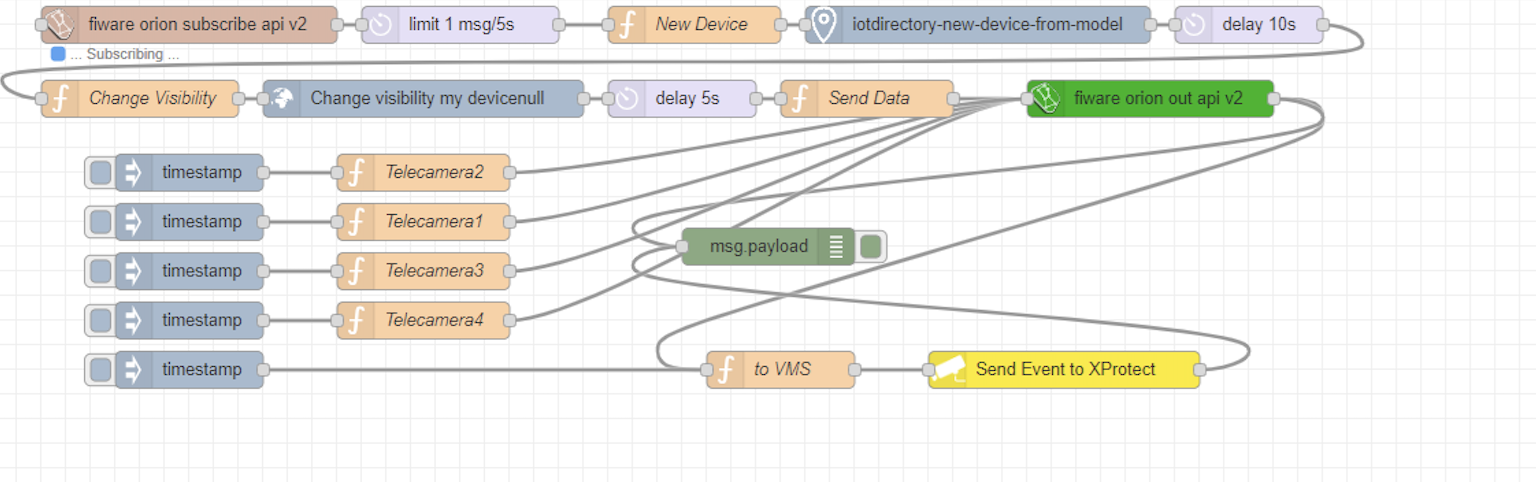
\includegraphics[width=1\linewidth]{img/S4CtoVMS.png}
    \caption{\textit{Flusso Node-RED per inviare eventi da S4C}}
    \label{14}
\end{figure}
\noindent
Grazie a questo flusso, il VMS viene aggiornato in tempo reale con gli eventi provenienti da Snap4City garantendo un aggiornamento immediato delle informazioni.
\subsection{Dal VMS a Snap4City}
Il secondo flusso di integrazione, che si vede in figura \ref{15}, è stato sviluppato per monitorare gli eventi generati dal VMS. Per simulare un canale di ascolto real-time è stato impostato un timer per attivare il blocco \textit{Print alert list from Xprotect} illustrato al capitolo \ref{receivevent}, che riceve una lista degli ultimi eventi creati sul VMS.
Una volta rilevato un nuovo evento con un flusso simile al precedente, viene creato un device di tipo \textit{AlertMilestone} su Snap4City, replicando in modo standardizzato le informazioni provenienti dal VMS.
Dopo aver fatto parsing dei dati ricevuti, il device viene quindi popolato con i dati dell’evento appena ricevuto e tali informazioni vengono automaticamente aggiunte a una tabella di monitoraggio sulla dashboard di Snap4City, accessibile agli operatori per visualizzare e modificare lo stato degli eventi.
\begin{figure}[H]
    \centering
    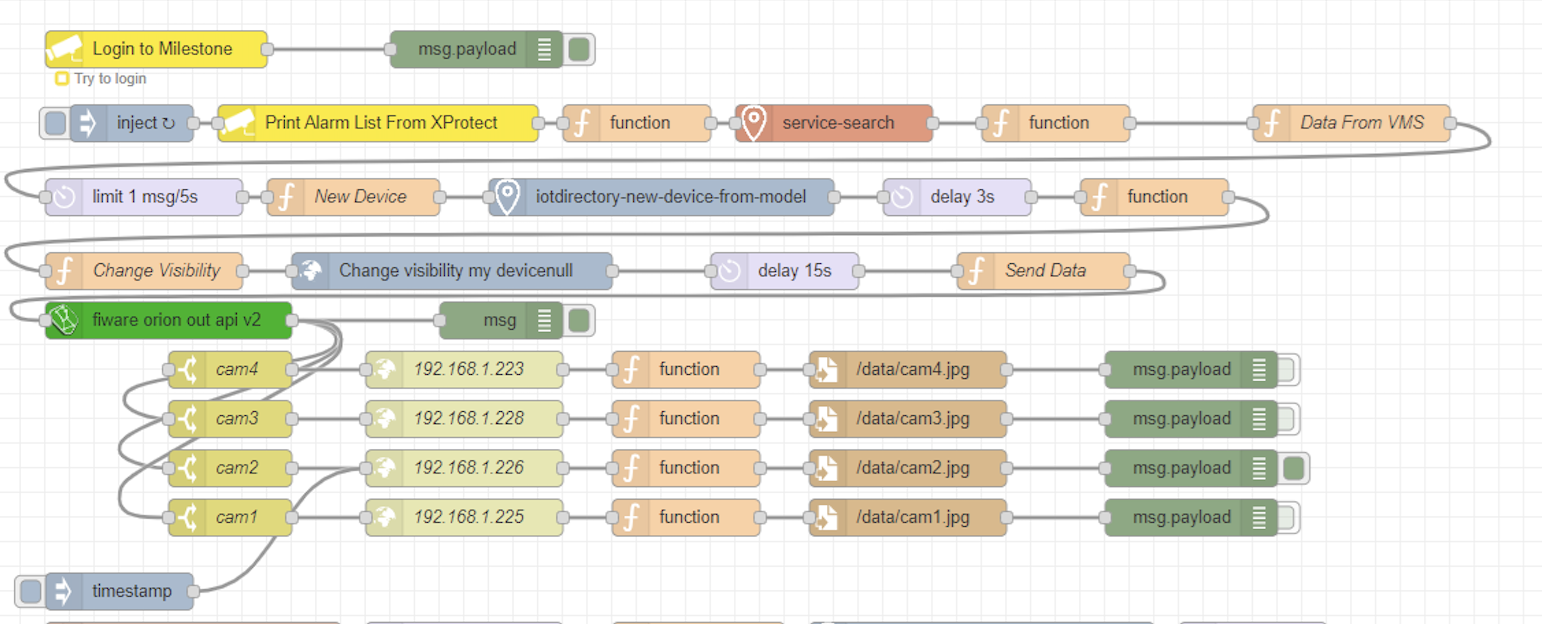
\includegraphics[width=1\linewidth]{img/VMStoS4C.png}
    \caption{\textit{Flusso Node-RED per ricevere eventi dal VMS}}
    \label{15}
\end{figure}
In sintesi, i flussi sviluppati costituiscono il ponte fondamentale per l’integrazione, consentendo uno scambio bidirezionale di dati in tempo reale. Questa sinergia migliora l’efficienza operativa, centralizza le informazioni e apre nuove opportunità per l’automazione e il monitoraggio avanzato, rendendo entrambe le piattaforme più efficaci nella gestione degli eventi e nella sicurezza urbana.

\section{Dashboard} \label{dashboard}
Le dashboard di Snap4City rappresentano un elemento centrale per l’interazione con il sistema, offrendo agli operatori strumenti intuitivi per la gestione e il monitoraggio degli eventi in tempo reale. Attraverso queste interfacce, è possibile registrare nuovi eventi, visualizzarne i dettagli, modificare i parametri associati e simulare scenari realistici per testare la risposta operativa.\\
Due dashboard principali sono state implementate per supportare le esigenze del sistema: la prima è dedicata alla registrazione degli eventi e alla visualizzazione contestuale tramite immagini delle telecamere, mentre la seconda consente la gestione dello stato e della gravità degli eventi, garantendo un controllo dinamico e immediato. \\
Un aspetto cruciale è rappresentato dai widget interattivi che compongono le dashboard, i quali includono mappe, pin per gli eventi, filtri, e immagini delle telecamere più vicine al punto di interesse selezionato. Questi componenti sono stati sviluppati utilizzando la \textit{Client-Side Business Logic} (CSBL) \cite{CSBL}, un approccio che sfrutta codice JavaScript per gestire eventi, connessioni e interazioni direttamente lato client. Grazie alla CSBL, i widget possono comunicare tra loro, rispondere in tempo reale alle azioni degli utenti e integrare dati provenienti da API esterne, fornendo un’esperienza d’uso fluida e reattiva. Questo approccio non solo riduce il carico computazionale sul server, ma permette anche di personalizzare l'interfaccia in base alle specifiche esigenze degli utenti, mantenendo elevata la flessibilità e la scalabilità del sistema.
\subsection{Registrazione Eventi} \label{regevent}

Questa dashboard permette agli operatori di creare manualmente nuovi eventi, specificandone i dettagli principali.
Al momento della creazione gli eventi sono in stato "init", e come si vede in figura \ref{16} è possibile selezionare la posizione sulla mappa dell'evento, che al click mostra le immagini in tempo reale della telecamera più vicina a quel punto. Inoltre la dashboard offre la possibilità di visualizzare sulla mappa luoghi e informazioni di interesse in tempo reale come la posizione di telecamere, ospedali oppure il flusso del traffico e il meteo. Questa funzionalità consente una valutazione rapida della situazione, facilitando decisioni operative informate.
Gli eventi registrati vengono visualizzati in una tabella che oltre ai dati sommari inseriti dall'operatore come la gravità e lo stato è arricchita da immagini catturate al momento della registrazione provenienti dalle telecamere, offrendo un contesto visivo immediato. Sulla mappa si possono applicare filtri agli eventi in base alla loro gravità e stato, consentendo agli operatori di ottenere una visione più chiara e mirata della situazione in specifiche aree di interesse.

\begin{figure}[H]
    \centering
    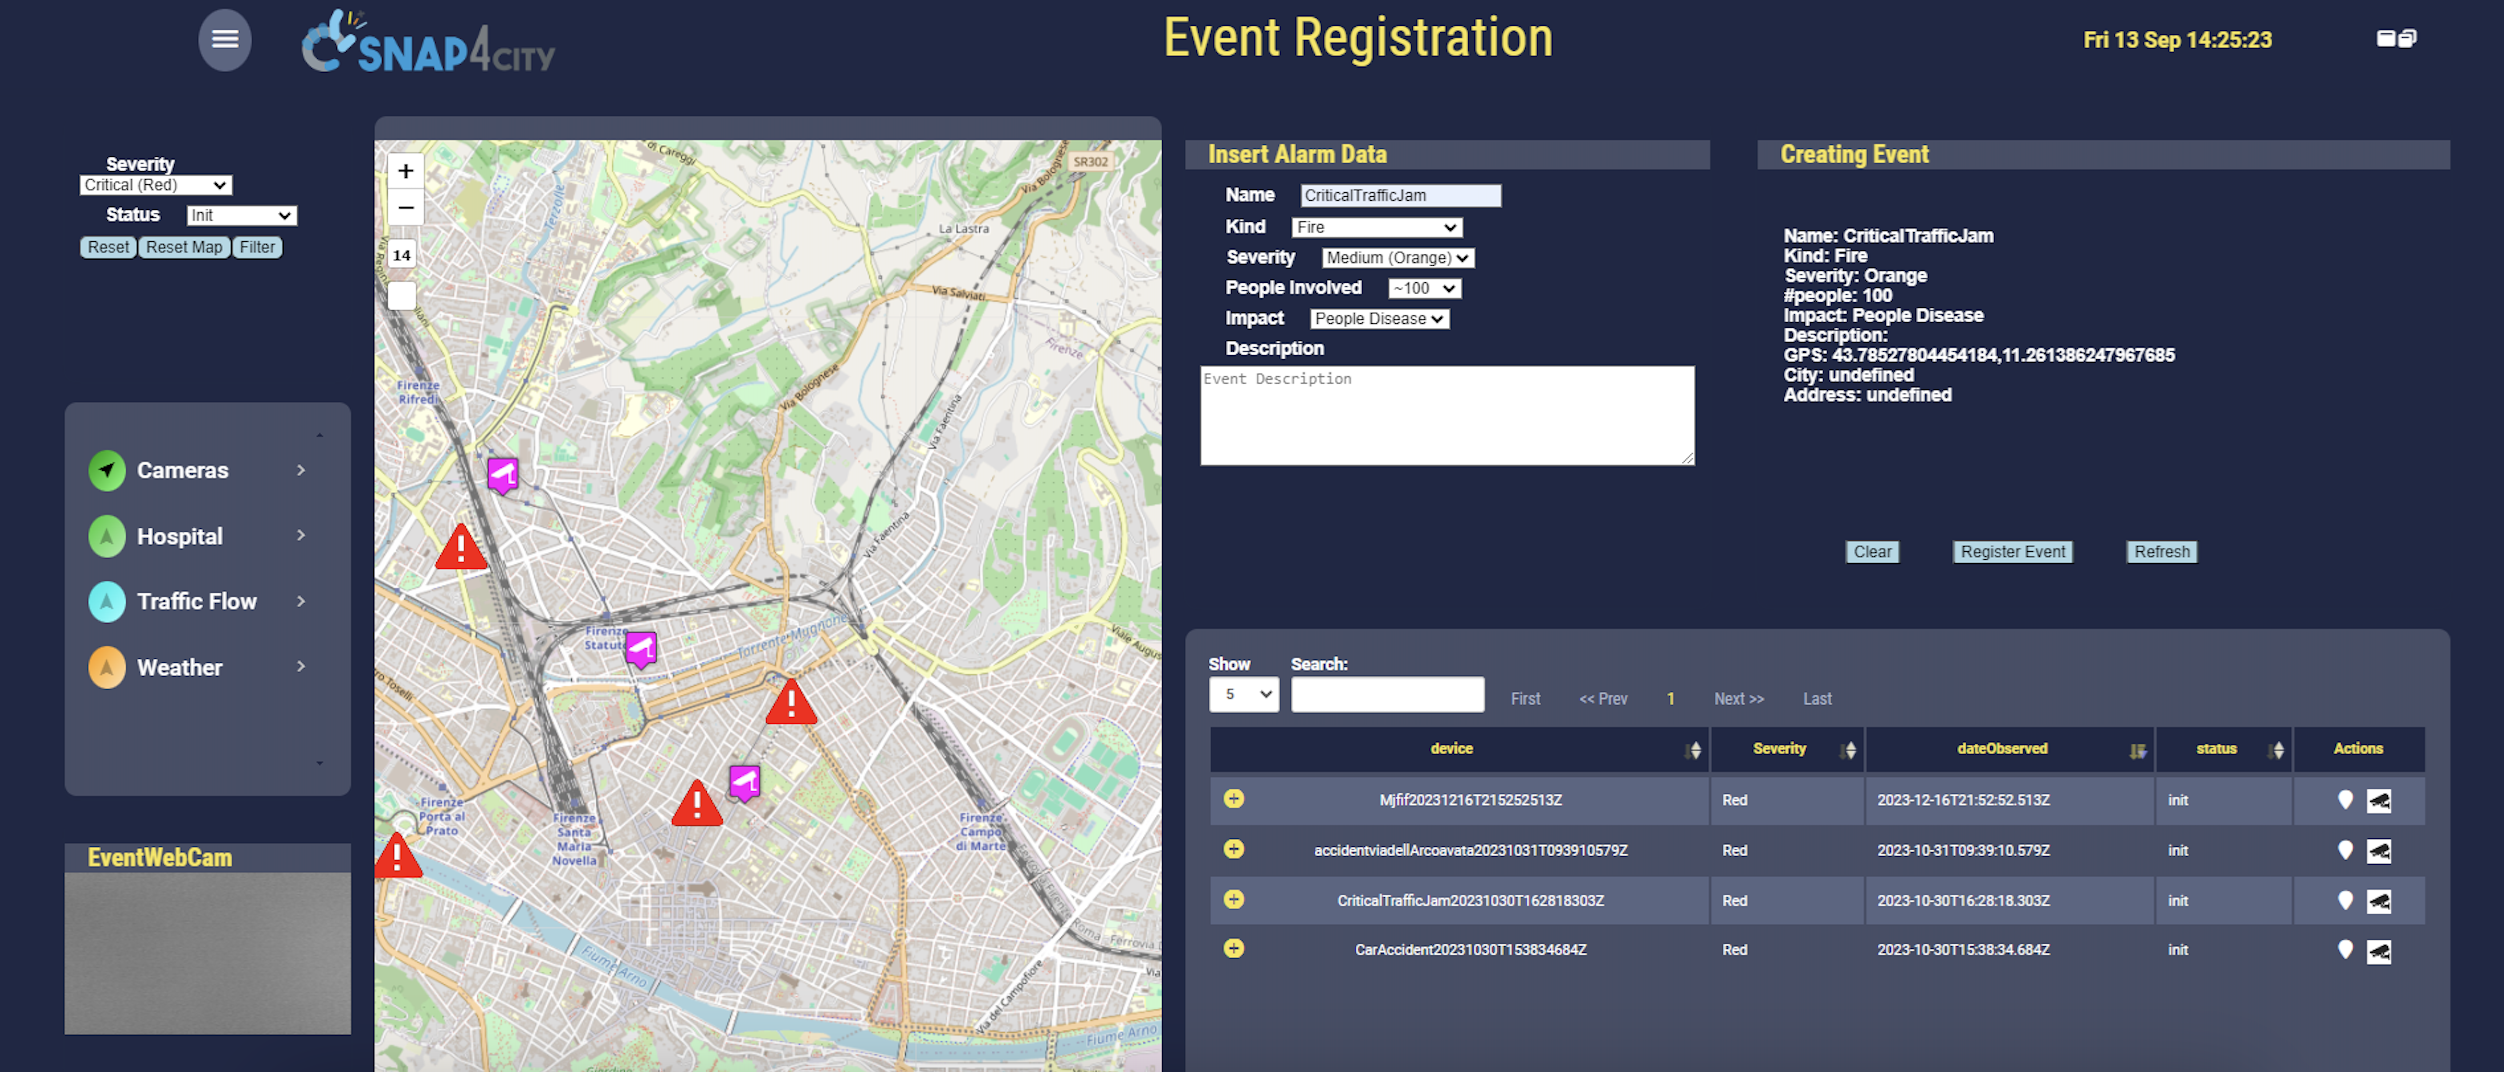
\includegraphics[width=1\linewidth]{img/EventRegistration.png}
    \caption{\textit{ Dashboard per registrazione eventi}}
    \label{16}
\end{figure}


\subsection{Gestione Stato ed Eventi}  

La seconda dashboard è stata sviluppata per consentire agli operatori di aggiornare lo stato e la severità degli eventi già registrati. Attraverso una tabella di monitoraggio, gli operatori possono visualizzare, filtrare e modificare i parametri associati a ciascun evento, garantendo un controllo dinamico e centralizzato. 
Questa funzionalità si rivela fondamentale per adattare le priorità in base all’evoluzione delle situazioni e migliorare la gestione delle risorse durante le emergenze. Inoltre, la possibilità di aggiornare i parametri in tempo reale assicura che le informazioni rimangano sempre allineate tra Snap4City e il VMS, ottimizzando la collaborazione tra le piattaforme.
\begin{figure}[H]
    \centering
    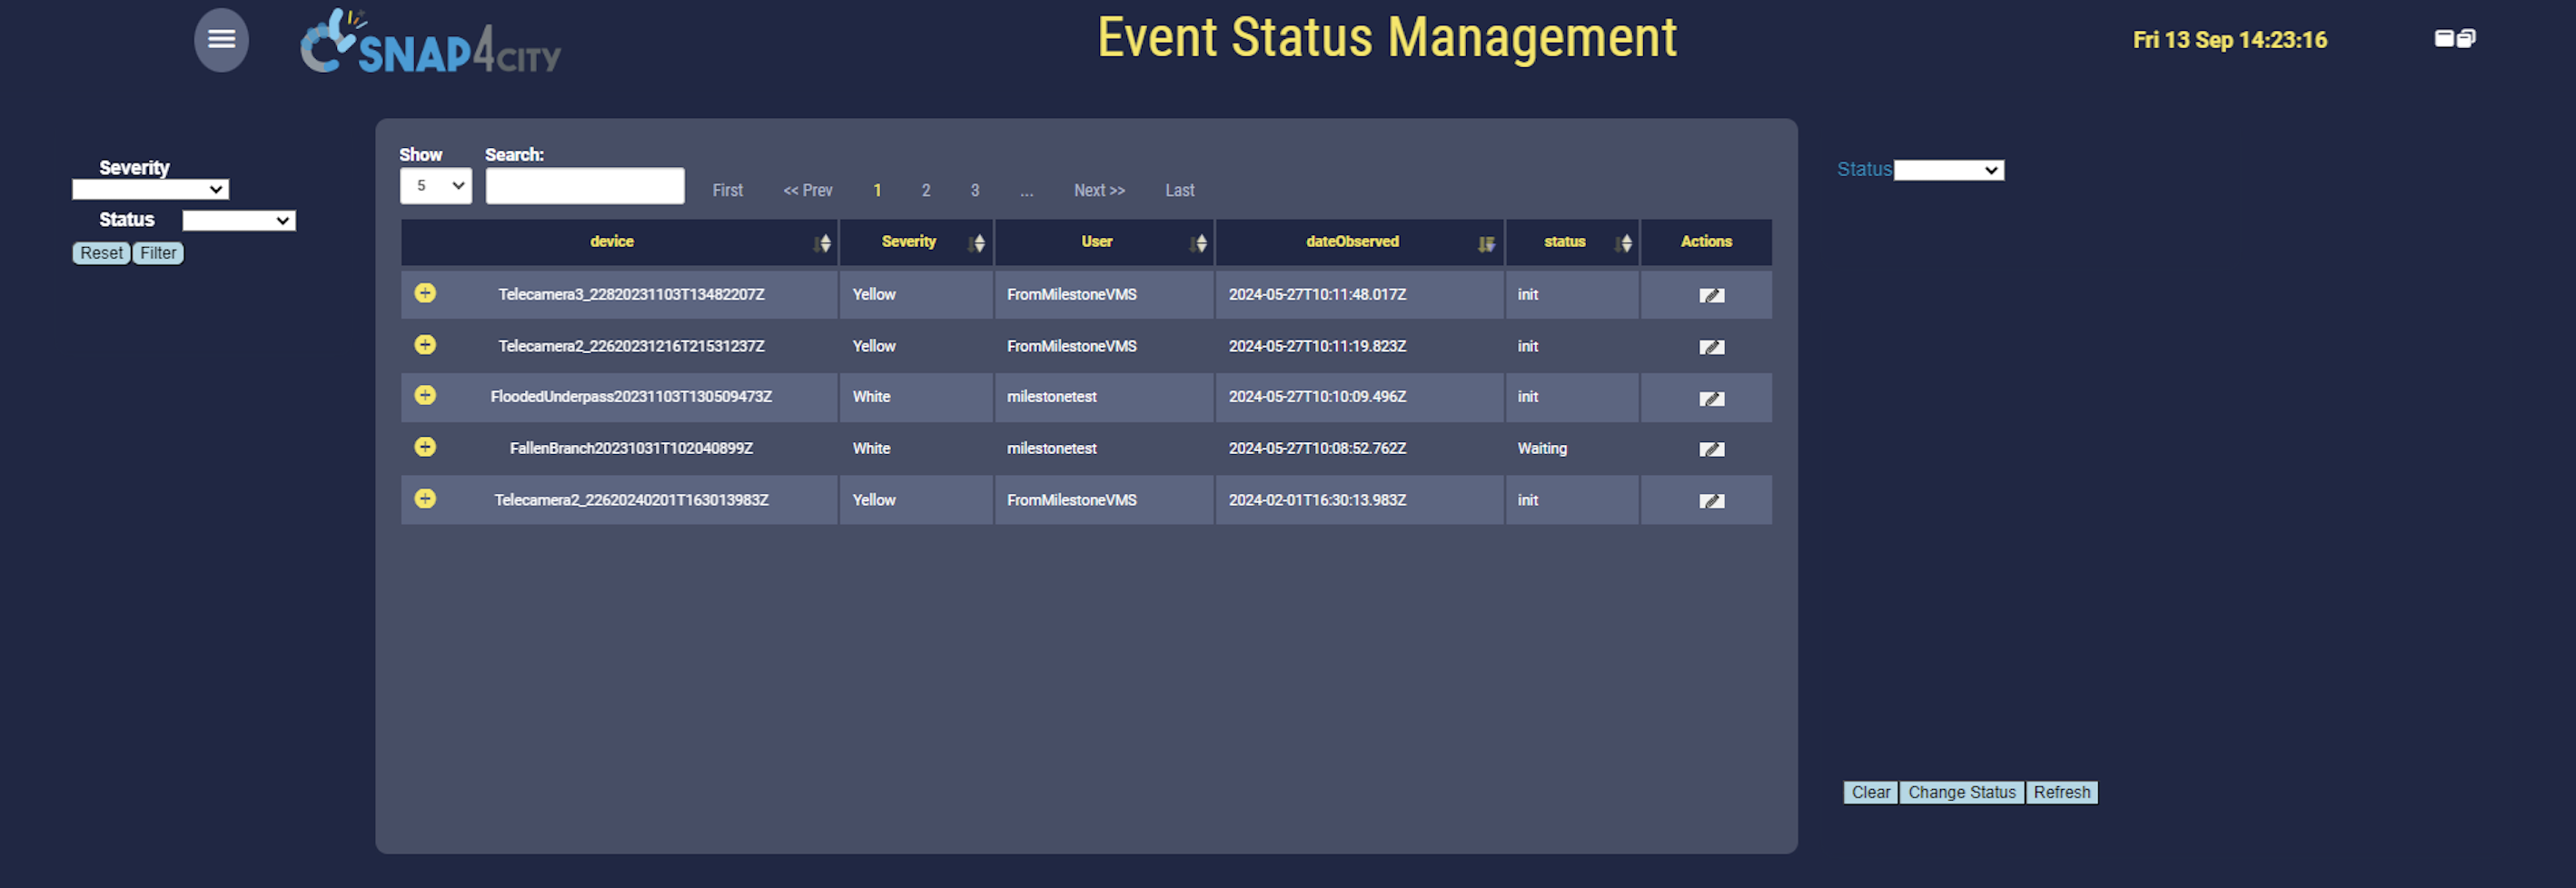
\includegraphics[width=1\linewidth]{img/EventStatus.png}
    \caption{\textit{ Dashboard per gestione eventi}}
    \label{17}
\end{figure}
\noindent
Queste due dashboard, integrate con i flussi descritti in precedenza, costituiscono il cuore operativo del sistema, garantendo agli operatori una gestione semplice, efficiente e scalabile degli eventi.  

\section{Video Management System (VMS)}
Attraverso le interfacce \textit{Management Client, Smart Client e Web Client} del VMS, gli operatori possono configurare le telecamere e gli eventi, monitorare le immagini in tempo reale e interagire con notifiche e allarmi. In questa sezione verranno descritte le funzionalità principali, soffermandosi sul processo di configurazione, sul monitoraggio degli eventi e su un tentativo di integrazione della dashboard all'interno dei client.

\subsection{Configurazione}

La configurazione del VMS permette di impostare le telecamere, definire eventi specifici e configurare allarmi personalizzati. Attraverso l'interfaccia, gli operatori possono aggiungere dispositivi, regolare parametri come risoluzione e posizione, e creare regole di attivazione per i vari eventi. \\
Le telecamere presenti nella stessa rete vengono rilevate automaticamente dal recording server, semplificando notevolmente il processo di configurazione. Nella figura \ref{18} è mostrata la schermata del Management Client che elenca le telecamere rilevate, accompagnata da un'anteprima video in diretta da ciascuna telecamera.
\begin{figure}[H]
    \centering
    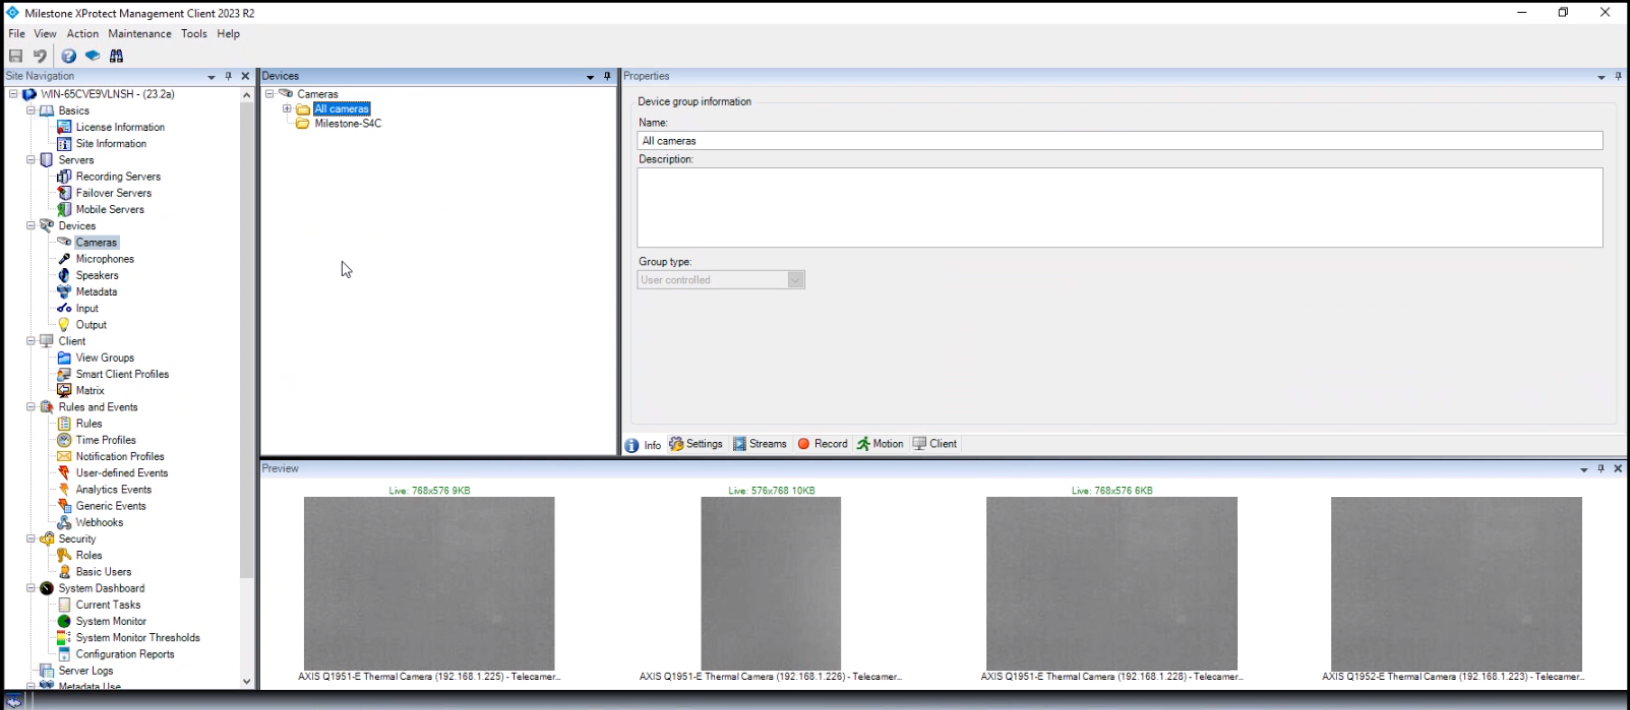
\includegraphics[width=1\textwidth]{img/cam list.png}
    \caption{Elenco telecamere con flusso video in diretta}
    \label{18}
\end{figure}
\noindent
Per quanto riguarda gli eventi sono stati definiti due tipi principali \textit{FromSnap4City} e \textit{FromVMS}. Il primo generato dalla dashboard di Snap4City, mentre il secondo generato direttamente dal VMS. Dopo aver definito gli eventi, è stato necessario configurare gli allarmi associati, mantenendo una corrispondenza uno-a-uno tra evento e allarme. Ogni evento analitico, infatti, è stato configurato per attivare il rispettivo allarme in modo da notificare gli operatori. 
Le figure \ref{19} e \ref{20} mostrano rispettivamente le schermate di configurazione degli eventi analitici e degli allarmi, evidenziandone i parametri principali.
\begin{figure}[H]
    \centering
    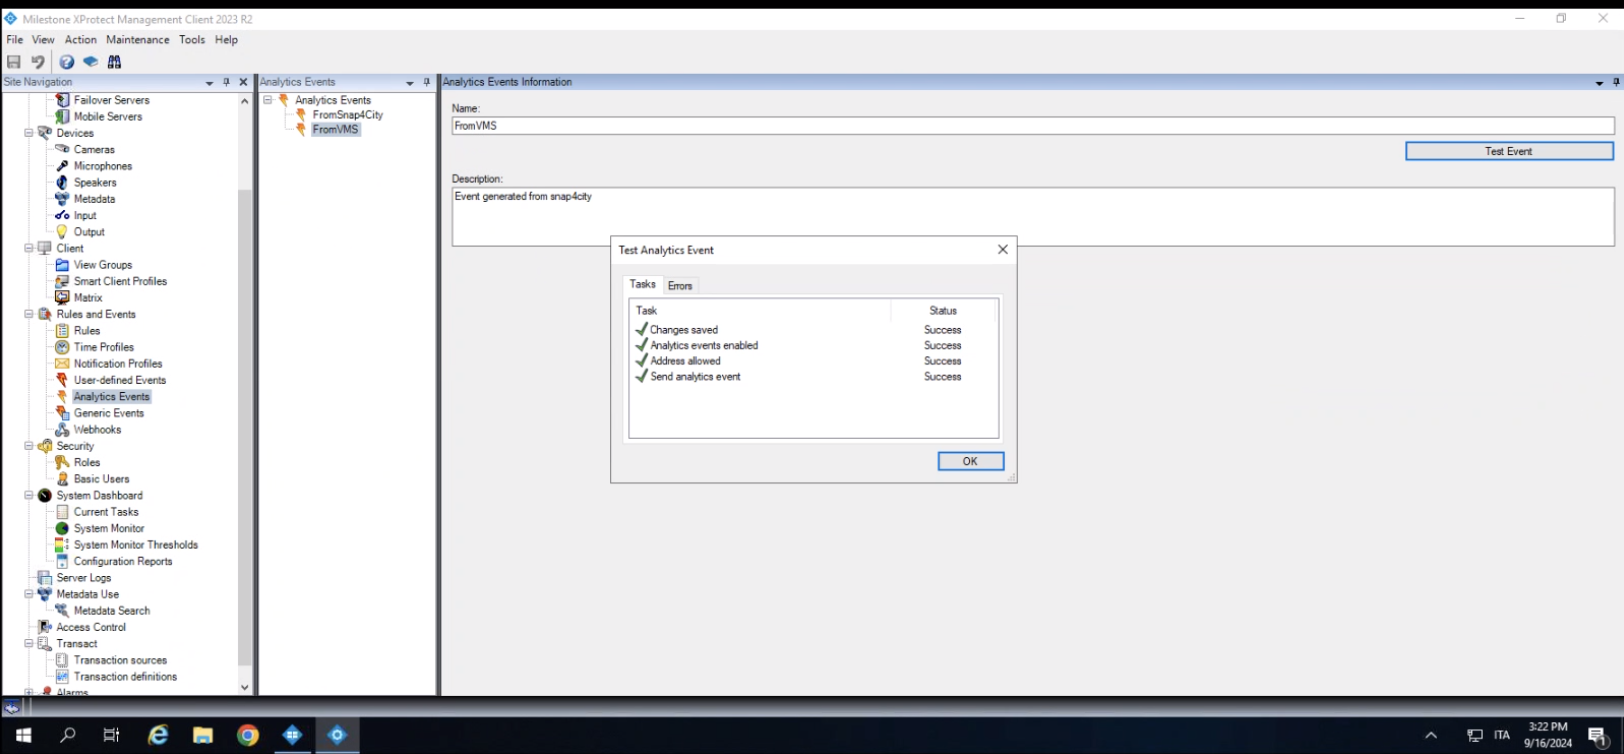
\includegraphics[width=1\textwidth]{img/analytics_event.png}
    \caption{Configurazione degli eventi analitici}
    \label{19}
\end{figure}
\begin{figure}[H]
    \centering
    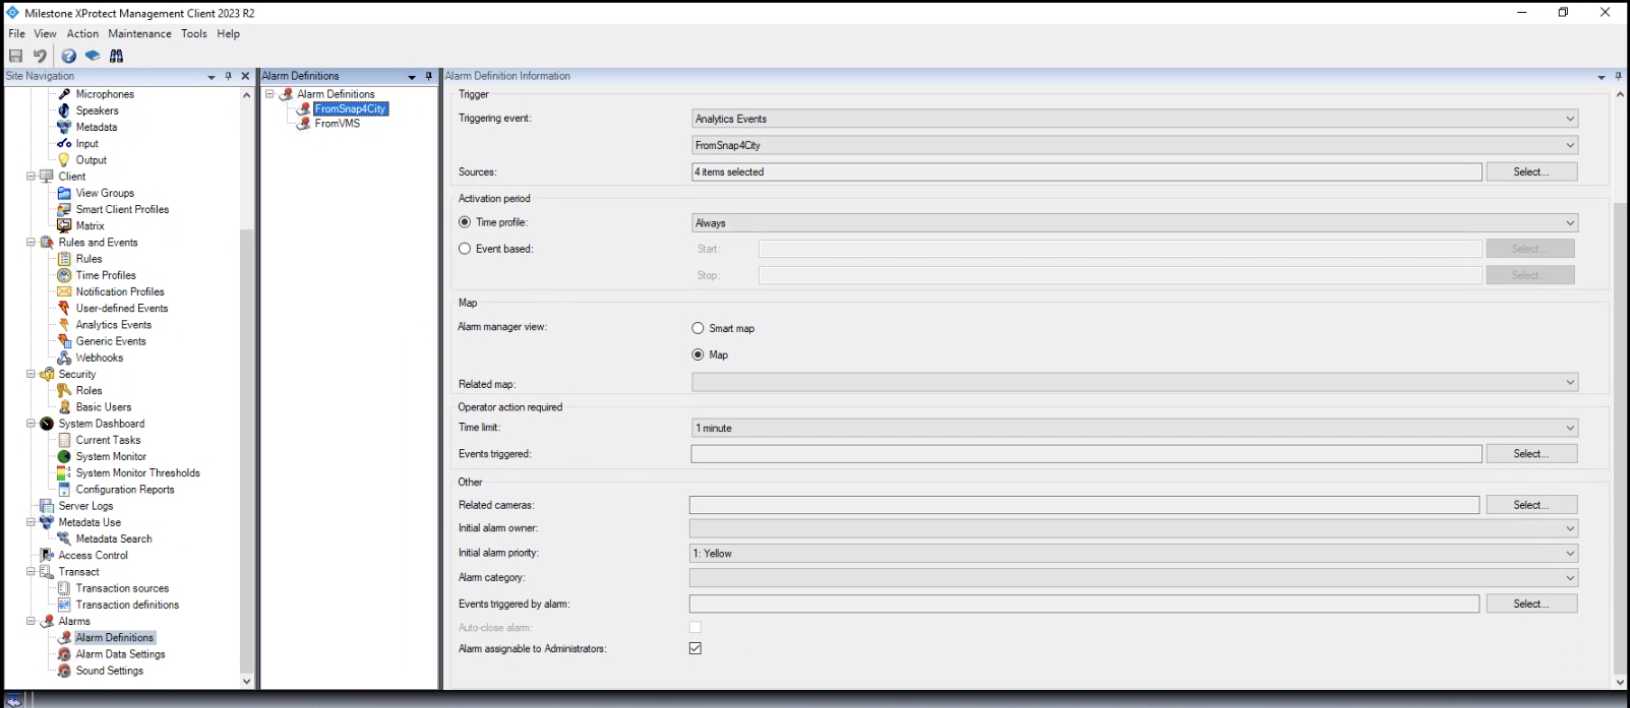
\includegraphics[width=1\textwidth]{img/alarm_def.png}
    \caption{Configurazione degli allarmi}
    \label{20}
\end{figure}

\subsection{Monitoraggio Eventi}

Il VMS consente di monitorare in tempo reale le immagini provenienti dalle telecamere e di gestire in modo efficace gli eventi e gli allarmi generati. L'interfaccia permette agli operatori di visualizzare notifiche immediate, analizzare gli eventi e intervenire rapidamente in caso di necessità, oltre che modificare i parametri degli allarmi come ad esempio la priorità, lo stato e la gravità. 
Di seguito nelle figure \ref{21} e \ref{22} vengono mostrate le interfacce di monitoraggio rispettivamente dello Smart Client e del Web Client.

\begin{figure}[H]
    \centering
    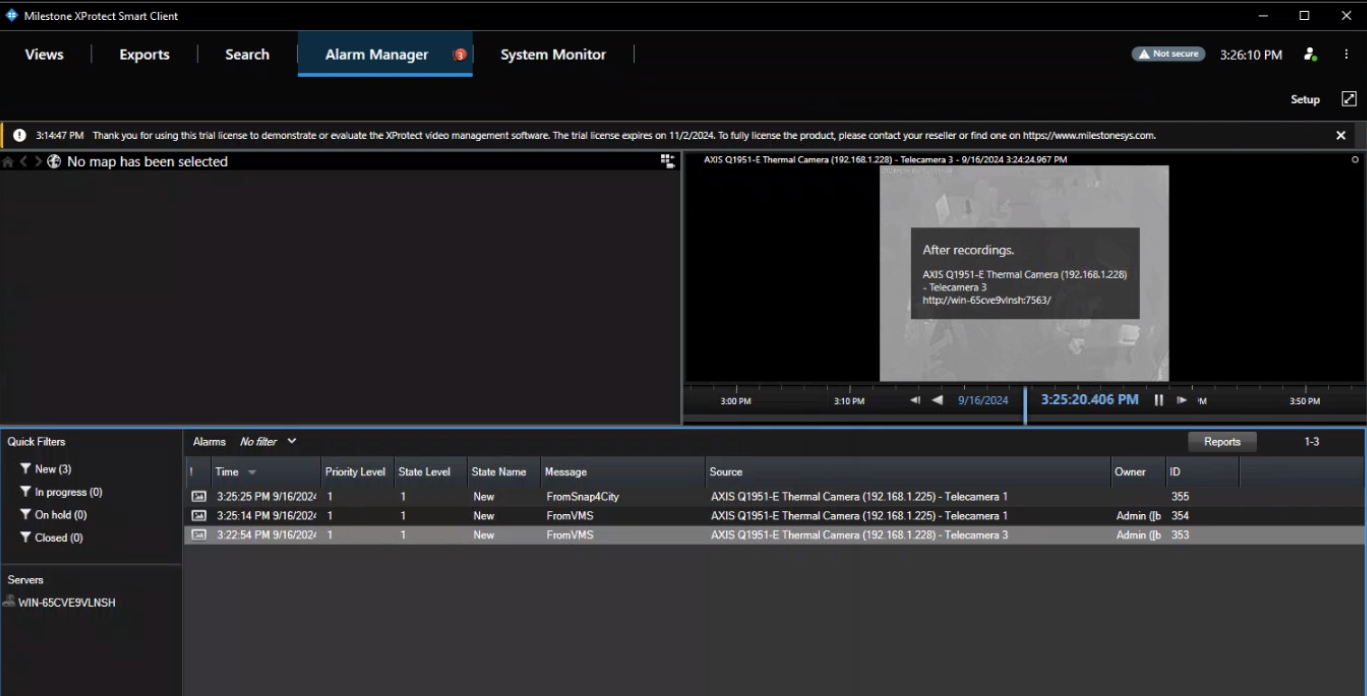
\includegraphics[width=1\textwidth]{img/alarm_client.png}
    \caption{Monitoraggio eventi su VMS Smart Client}
    \label{21}
\end{figure}
\begin{figure}[H]
    \centering
    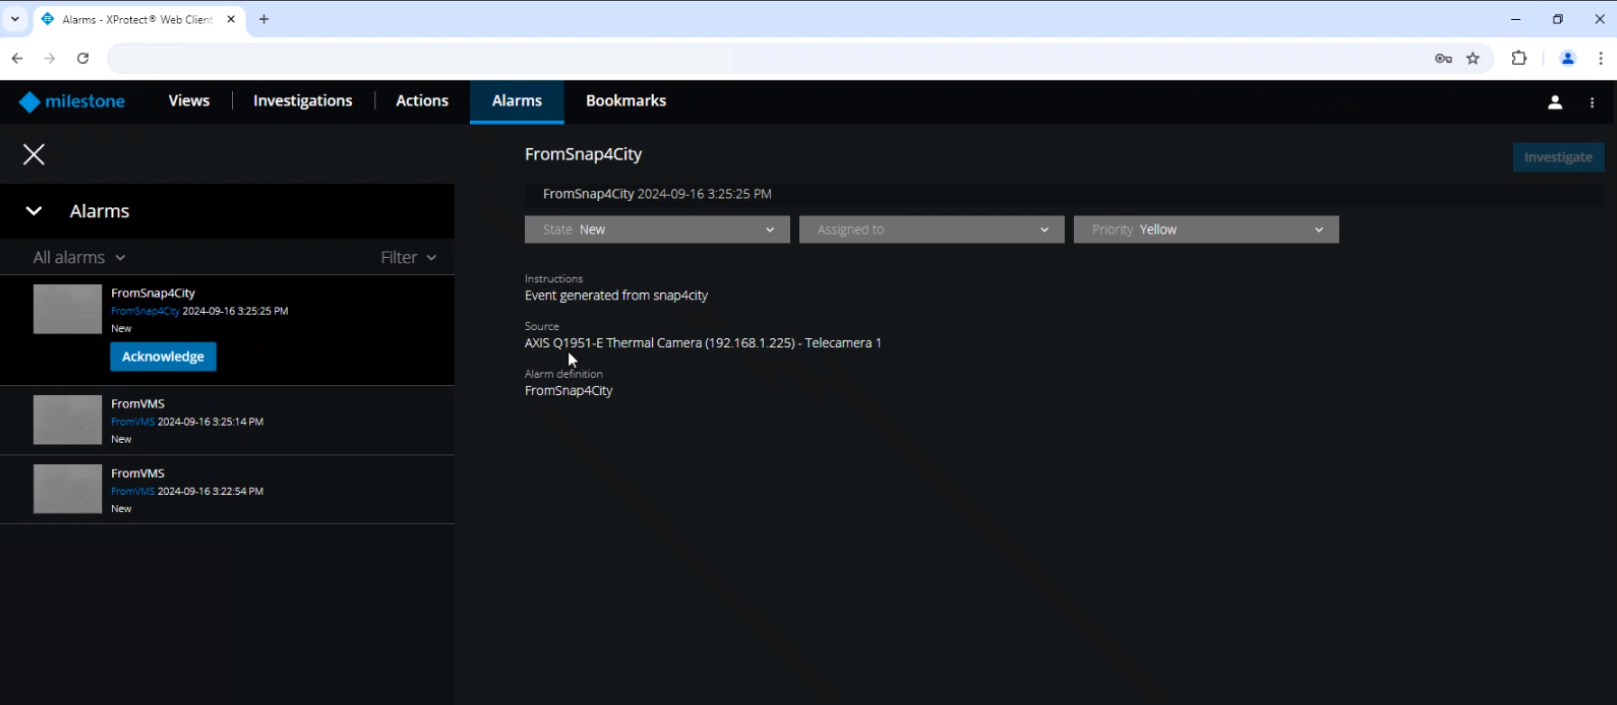
\includegraphics[width=1\textwidth]{img/alarm_client_web.png}
    \caption{Monitoraggio eventi su VMS Web Client}
    \label{22}
\end{figure}


\subsection{Tentativo di Integrazione nei Client}

Durante lo sviluppo, è stato effettuato un tentativo per integrare le dashboard descritte nella sezione \ref{dashboard} direttamente all'interno dei due client del VMS, sfruttando la sezione \textit{Views}. Questa soluzione avrebbe permesso di combinare in un'unica interfaccia le funzionalità di monitoraggio delle telecamere con quelle analitiche della dashboard, ma sono emerse alcune limitazioni tecniche del VMS. \\
Il \textit{Web Client} non supporta l'integrazione di pagine web esterne, mentre lo \textit{Smart Client} non riesce a eseguire correttamente le funzionalità JavaScript necessarie per il pieno funzionamento della dashboard con i vari widget CSBL, in quanto consente l'embedding ma tramite un browser obsoleto (Windows Explorer 11). Questo rende l'integrazione statica e praticamente non utilizzabile.
Nelle figure \ref{23} e \ref{24} vengono mostrati i risultati del tentativo di integrazione sia per lo Smart che per il Web client.

\begin{figure}[H]
    \centering
    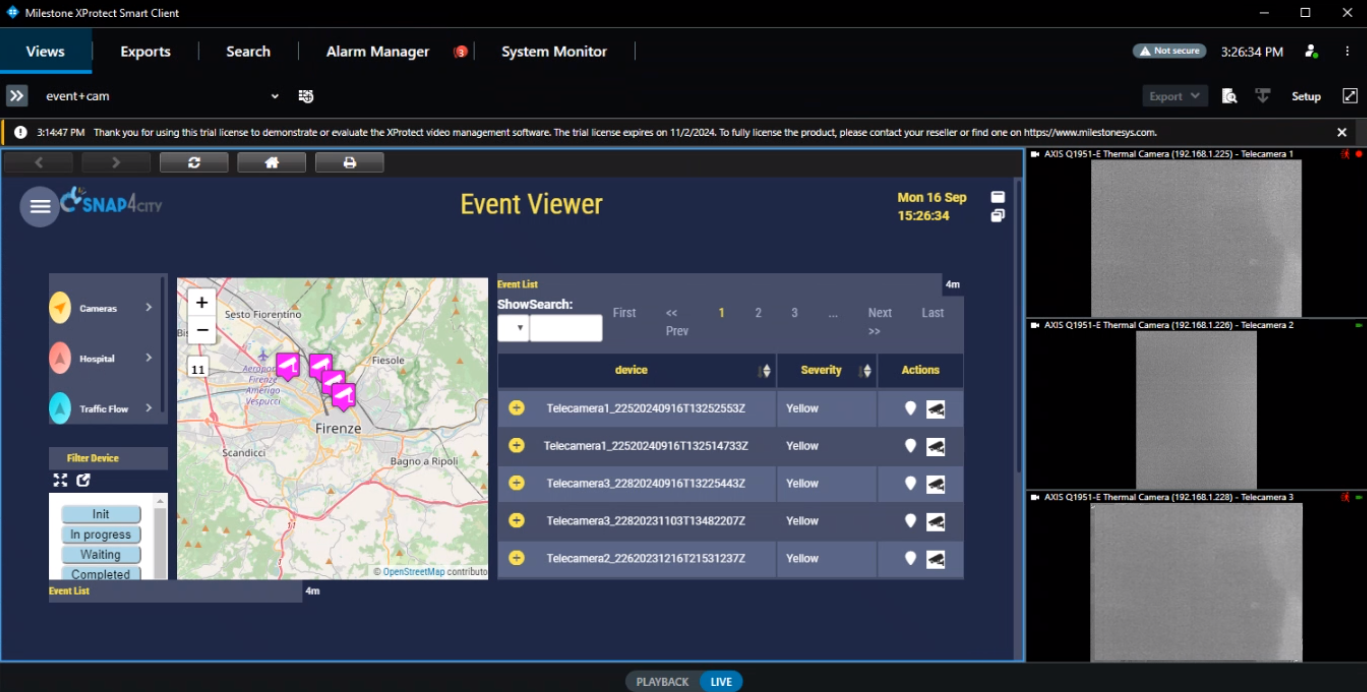
\includegraphics[width=1\textwidth]{img/viewclient.png}
    \caption{Test integrazione dashboard in Smart Client}
    \label{23}
\end{figure}
\begin{figure}[H]
    \centering
    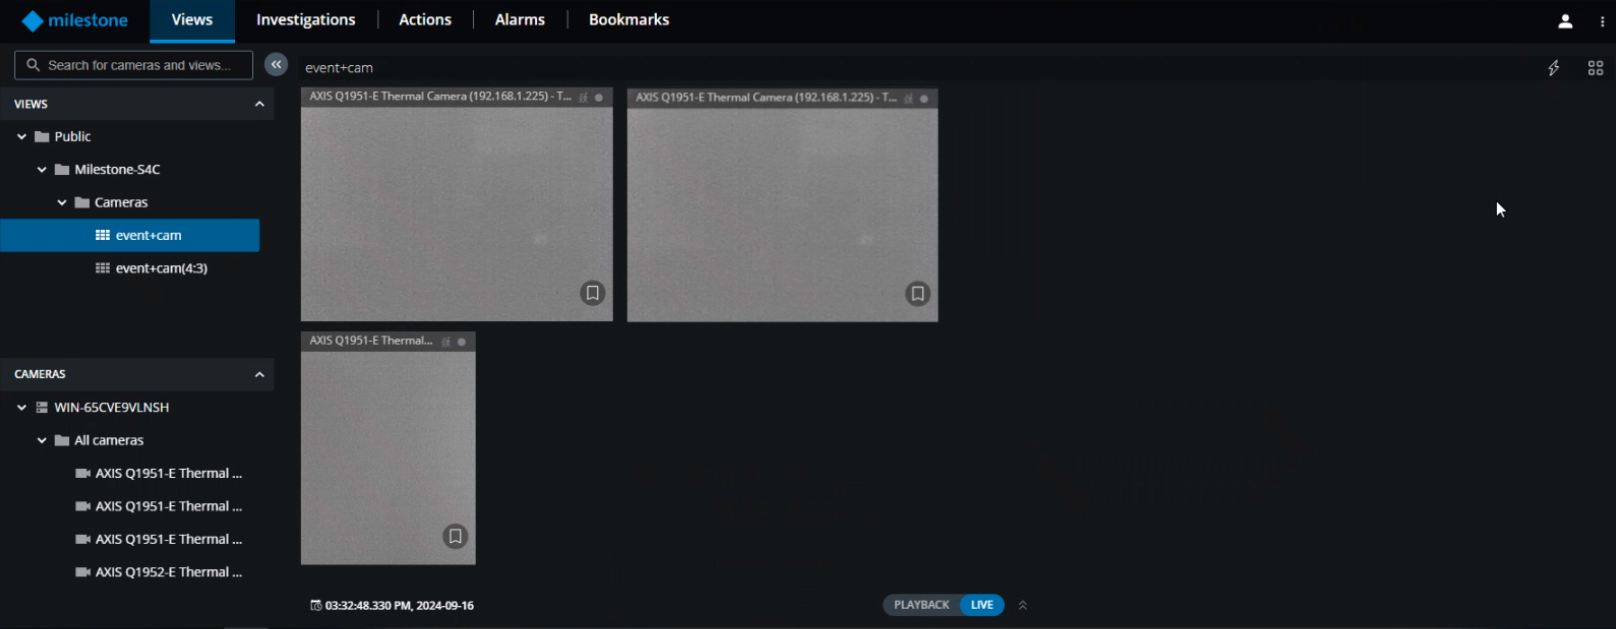
\includegraphics[width=1\textwidth]{img/viewweb.png}
    \caption{Test integrazione dashboard in Web Client}
    \label{24}
\end{figure}
\noindent
Sebbene il tentativo non abbia avuto esito positivo, rappresenta comunque un'importante esplorazione delle potenzialità e dei limiti del sistema di Milestone, fornendo spunti per futuri sviluppi.

\chapter{Test e Validazione}
In questo capitolo vengono descritti i test condotti per verificare il corretto funzionamento dell’integrazione tra Snap4City e il VMS di Milestone. L’obiettivo principale di queste prove è stato accertare che i due sistemi potessero comunicare correttamente, garantendo la trasmissione e la visualizzazione degli eventi di sicurezza.

\section{Generazione di un Evento da Snap4City}
Uno degli aspetti chiave della verifica ha riguardato la capacità di Snap4City di generare un evento e trasmetterlo correttamente al VMS di Milestone. Per simulare questa situazione, è stato testato il flusso di creazione di un evento direttamente dalla dashboard di Snap4City, utilizzando la mappa interattiva per selezionare una posizione specifica e associarvi una telecamera nelle vicinanze. Una volta creato l’evento con i parametri desiderati, il sistema ha inviato le informazioni tramite Node-RED al VMS, che le ha ricevute e archiviate nel proprio database. La verifica si è basata sulla corretta comparsa dell’evento all’interno dell’interfaccia client del VMS e sulla capacità di Snap4City di mostrare il feed della telecamera associata in tempo reale. L’esito positivo del test è stato confermato dalla presenza dell’evento nella piattaforma di Milestone con tutti i dettagli corretti e dalla possibilità di visualizzare il flusso video della telecamera selezionata.

\section{Ricezione di un Evento dal VMS}
Un altro test fondamentale ha riguardato la capacità di Snap4City di ricevere e visualizzare eventi generati direttamente dal VMS di Milestone. Per verificarlo, è stato creato un evento di allarme all'interno del VMS, includendo informazioni come la descrizione, il livello di criticità e l’identificativo della telecamera coinvolta. Attraverso il flusso di integrazione basato su Node-RED, l’evento è stato trasmesso a Snap4City, che ha provveduto a rappresentarlo sulla propria dashboard. Qui, l’allarme è stato mostrato su una tabella dedicata, con tutti i dettagli necessari, e sulla mappa interattiva, dove un’icona ne ha segnalato la posizione, facilitando l’identificazione della criticità. L’integrazione ha funzionato come previsto: l’evento generato nel VMS è stato visualizzato correttamente in Snap4City, e l’interfaccia ha aggiornato in tempo reale la lista degli allarmi. Inoltre, è stato possibile consultare il feed video della telecamera associata, confermando che le informazioni fossero correttamente instradate tra i due sistemi.

Questi test hanno permesso di verificare che l’integrazione tra Snap4City e il VMS di Milestone funziona come previsto, garantendo il trasferimento e la visualizzazione degli eventi senza anomalie. Sebbene non sia stata effettuata una simulazione operativa in un contesto reale, il sistema ha dimostrato di poter gestire correttamente gli eventi e le relative informazioni, offrendo agli operatori uno strumento efficace per il monitoraggio e la gestione della sicurezza urbana.
\chapter{CONCLUSIONI}

In questa tesi è stato affrontato il processo di integrazione tra Snap4City, una piattaforma di smart city, e il Video Management System (VMS) di Milestone. L'obiettivo principale era migliorare la gestione e l'analisi dei dati provenienti dalle telecamere termiche, consentendo un monitoraggio più efficace e una risposta tempestiva agli eventi rilevanti sul territorio. L'integrazione è stata realizzata attraverso la progettazione di modelli specifici in Snap4City e l'utilizzo di flussi Node-RED per garantire una comunicazione bidirezionale tra Snap4City e il VMS di Milestone.

\section{Sintesi dei Risultati}

\subsection{Progettazione dei Modelli}
Sono stati sviluppati tre modelli chiave all'interno di Snap4City:
\textit{MilestoneCam} utilizzato per rappresentare le telecamere, includendo attributi come l'indirizzo IP e il CamID per l'identificazione delle sorgenti video.
\textit{AlertMilestone} progettato per ricevere e gestire eventi di allarme generati dal VMS e popolare in modo efficace la dashboard di Snap4City con i dettagli dell’evento e il feed video della telecamera.
\textit{AlertListener} che permette di generare eventi direttamente dalla dashboard di Snap4City, inviandoli al VMS tramite i flussi Node-RED, per assicurare che possano essere visualizzati e gestiti nel client del VMS.

\subsection{Integrazione e Automazione}
L'uso di flussi di automazione in Node-RED ha permesso di configurare la gestione bidirezionale degli eventi, che in questo contesto ha svolto il ruolo di middleware avanzato, facilitando l’invio e la ricezione di eventi tra Snap4City e il VMS. Questo approccio ha permesso di rispondere prontamente agli eventi e di gestire le notifiche in tempo reale.
Inoltre, è stata implementata la Client-Side Business Logic (CSBL) per rendere i widget della dashboard interattivi lato client. Questo ha migliorato l’esperienza utente, permettendo una gestione più dinamica e reattiva delle interfacce senza la necessità di continue richieste al server. L’integrazione della CSBL ha consentito di ottimizzare le prestazioni della dashboard, riducendo la latenza e migliorando l’usabilità complessiva del sistema.

\section{Limitazioni Riscontrate}
Durante il progetto, sono state riscontrate alcune limitazioni tecniche legate all'architettura del VMS di Milestone, la principale è a livello di personalizzazione e di integrazione con componenti esterni. Sebbene il client desktop sia idoneo per la visualizzazione degli eventi inviati da Snap4City, il web client offre una gestione molto limitata e non consente di integrare direttamente la dashboard di Snap4City, costringendo gli operatori a utilizzare interfacce multiple.
\section{Sviluppi Futuri}
Per potenziare ulteriormente l'integrazione tra Snap4City e il VMS di Milestone, si possono esplorare diversi sviluppi futuri:
\begin{itemize}
    \item \textbf{Espansione del Middleware:} Node-RED potrebbe essere ulteriormente arricchito con funzionalità che permettano una sincronizzazione più automatica e completa tra i due sistemi, sviluppando nuovi blocchi in modo da ridurre la necessità di configurazioni manuali e migliorare la reattività agli eventi in tempo reale.
    \item \textbf{Sviluppo di un’Interfaccia Unificata:} Creare un’interfaccia web che integri le funzionalità principali del VMS e della dashboard Snap4City, permettendo una vista centralizzata per la gestione degli eventi e il monitoraggio delle telecamere, eliminando il passaggio tra le piattaforme.
    \item  \textbf{Supporto per il Client Web VMS:} Collaborare con i fornitori del VMS per estendere il supporto alle funzionalità di personalizzazione nel client web e consentire il miglioramento della gestione degli eventi in un contesto multi-interfaccia.
    \item \textbf{Integrazione di Analisi Predittiva e AI:} Integrare algoritmi di analisi predittiva per analizzare i flussi video e identificare automaticamente comportamenti sospetti, generando notifiche in Snap4City senza bisogno di supervisione continua.
\end{itemize}


\afterpage{\blankpage}


\begin{thebibliography}{9}
\bibitem{snap4city}
\emph{Snap4City: \\}
\url{https://www.snap4city.org/}

\bibitem{milestoneVMS}
\emph{Milestone Xprotect: \\}
\url{https://www.milestonesys.com/it/products/software/xprotect/}

\bibitem{snap}
\textsc{C. Badii, E. G. Belay, P. Bellini, D. Cenni, M. Marazzini, M. Mesiti, P. Nesi, G. Pantaleo, M. Paolucci, S. Valtolina, M. Soderi, I. Zaza}, 
\emph{Snap4City: A Scalable IOT/IOE Platform for Developing Smart City Applications}, 
Int. Conf. IEEE Smart City Innovation, Cina 2018, IEEE Press.\\
\url{https://ieeexplore.ieee.org/document/8560331}

\bibitem{nodered}
\emph{Node-RED: \\}
\url{ https://nodered.org}

\bibitem{xprotect-version}
\emph{Versioni di XProtect: \\}
\url{https://www.milestonesys.com/products/software/xprotect-comparison}

\bibitem{requirements}
\emph{Requisiti per XProtect: \\}
\url{https://www.milestonesys.com/systemrequirements}

\bibitem{SQLserver}
\emph{Documentazione Microsoft SQL Server: \\}
\url{https://learn.microsoft.com/en-us/sql/sql-server/?view=sql-server-ver16}

\bibitem{.NET}
\emph{Documentazione .NET Framework: \\}
\url{https://learn.microsoft.com/en-us/dotnet/framework/}

\bibitem{failover}
\emph{Documentazione Server di Failover: \\}
\url{https://doc.milestonesys.com/latest/en-US/portal/htm/chapter-page-failoverms.htm}

\bibitem{mipdoc}
\emph{Documentazione MIP: \\}
\url{https://doc.developer.milestonesys.com/mipvmsapi}

\bibitem{smartclient}
\emph{Documentazione Smart Client: \\}
\url{https://doc.milestonesys.com/latest/en-US/portal/htm/chapter-page-sc.htm}

\bibitem{sdk}
\emph{Documentazione MIP SDK: \\}
\url{https://www.milestonesys.com/it/support/for-developers/sdk}

\bibitem{webclient}
\emph{Documentazione Web Client: \\}
\url{https://doc.milestonesys.com/latest/en-US/portal/htm/chapter-page-webc.htm}

\bibitem{noderedmilestone}
\emph{Documentazione S4C-Milestone: \\}
\url{https://flows.nodered.org/node/node-red-contrib-snap4city-milestone}

\bibitem{eventdoc}
\emph{Documentazione di invio eventi al VMS: \\}
\url{https://download.milestonesys.com/MIPSDK/Samples/TriggerAlarmFromExternal-ConceptSolution.pdf}

\bibitem{RestAPIdoc}
\emph{Documentazione per RESTful API: \\}
\url{https://doc.developer.milestonesys.com/mipvmsapi/api/config-rest/v1/}

\bibitem{SoapAPIdoc}
\emph{Documentazione per SOAP API: \\}
\url{https://doc.developer.milestonesys.com/html/index.html?base=serversoaphelp/index.html&tree=tree_3.html}

\bibitem{CSBL}
\emph{Documentazione Client Side Business Logic Widget: \\}
\url{https://www.snap4city.org/drupal/node/911}

\bibitem{integrationsnap}
\emph{Pagina web del progetto: \\}
\url{https://www.snap4city.org/drupal/node/966}

\end{thebibliography}

\end{document}